\documentclass[10pt, compress]{beamer}

\usetheme[numbering=fraction, progressbar=none, titleformat=smallcaps, sectionpage=none]{metropolis}
\usepackage{booktabs}
\usepackage{array}
\usepackage{listings}
\usepackage{graphicx}
\usepackage[brazilian]{babel}
\usepackage[scale=2]{ccicons}
\usepackage{url}
\usepackage{relsize}
\usepackage{wasysym}

\usepackage{pgfplots}
\usepgfplotslibrary{dateplot}

\lstset{ %
  backgroundcolor={},
  basicstyle=\ttfamily\footnotesize,
  breakatwhitespace=true,
  breaklines=true,
  captionpos=n,
  commentstyle=\color{orange},
  escapeinside={\%*}{*)},
  extendedchars=true,
  frame=n,
  keywordstyle=\color{orange},
  language=C++,
  rulecolor=\color{black},
  showspaces=false,
  showstringspaces=false,
  showtabs=false,
  stepnumber=2,
  stringstyle=\color{gray},
  tabsize=2,
  keywords={thrust,plus,device_vector, copy,transform,begin,end, copyin,
  copyout, acc, \_\_global\_\_, void, int, float, main, threadIdx, blockIdx,
  blockDim, if, else, malloc, NULL, cudaMalloc, cudaMemcpy, cudaSuccess,
  cudaGetLastError, cudaDeviceSynchronize, cudaFree, cudaMemcpyDeviceToHost,
  cudaMemcpyHostToDevice, const, data, independent, kernels, loop,
  fprintf, stderr, cudaGetErrorString, EXIT_FAILURE, for, dim3},
  otherkeywords={::, \#pragma, \#include, <<<,>>>, \&, \*, +, -, /, [, ], >, <}
}

\renewcommand*{\UrlFont}{\ttfamily\smaller\relax}

\graphicspath{{../img/}}

\title{Introdução à Programação de GPUs \\ com a Plataforma CUDA}
\author{\footnotesize Pedro Bruel \\ {\scriptsize phrb@ime.usp.br}}
\institute{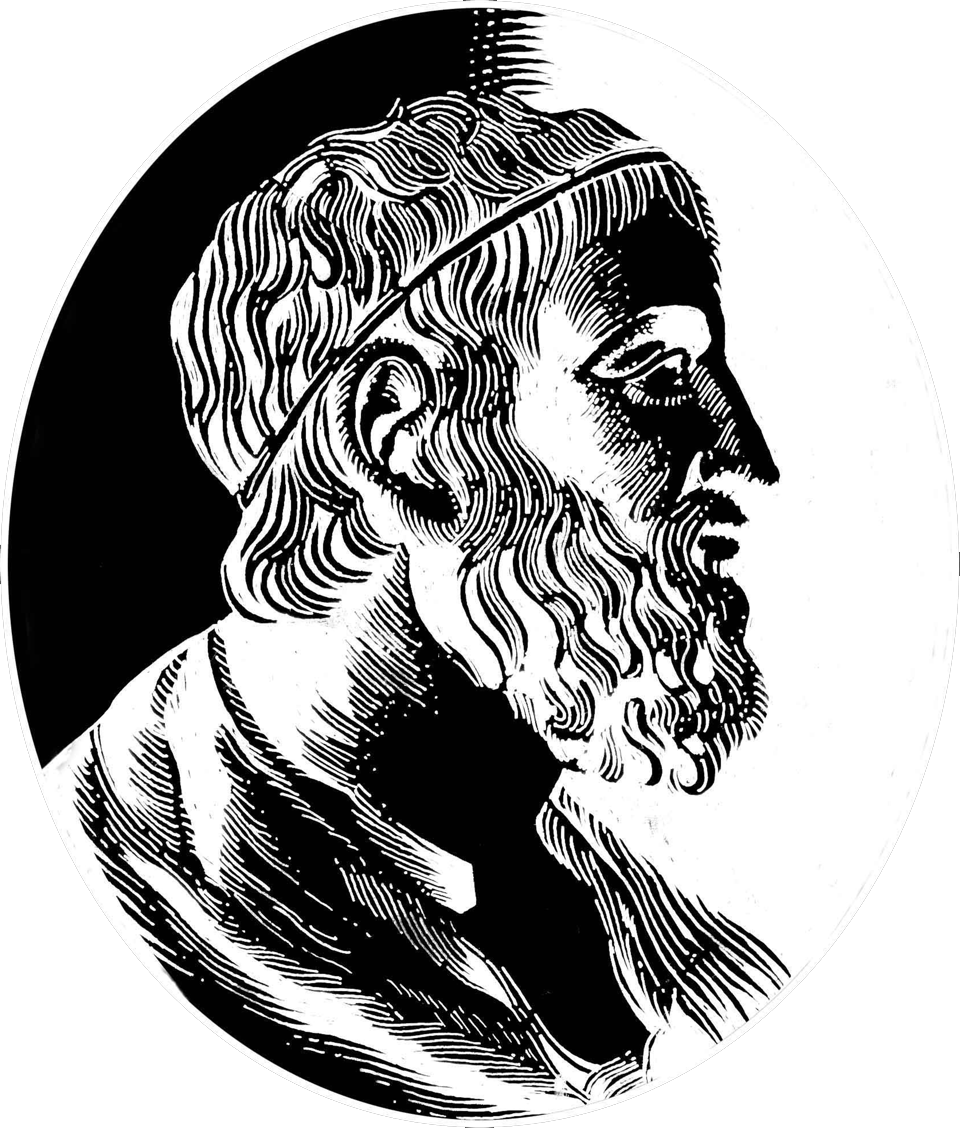
\includegraphics[height=2cm]{imelogo}\\[0.2cm] Instituto de Matemática e Estatística \\ Universidade de São Paulo}
\date{\scriptsize 04 de Agosto de 2016}

\begin{document}

\part{Parte I}

\maketitle

\section{Introdução}

\subsection{Sobre}

\begin{frame}
    \frametitle{Sobre}
    \begin{columns}[T,onlytextwidth]
        \column{0.5\textwidth}
        \begin{center}
            
\includegraphics[width=.45\textwidth]{pedro}

            Pedro Bruel
        \end{center}

        \begin{itemize}
            \item \alert{phrb}@ime.usp.br
            \item \url{www.ime.usp.br/~phrb}
            \item \url{github.com/phrb}
        \end{itemize}

        \column{0.5\textwidth}
        \begin{center}
            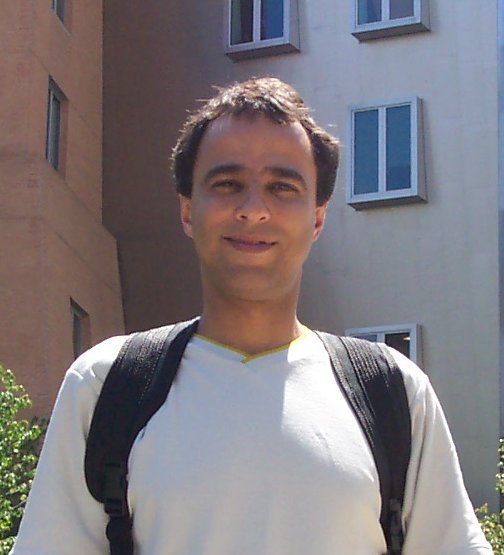
\includegraphics[width=.4\textwidth]{alfredo}

            Alfredo Goldman
        \end{center}

        \begin{itemize}
            \item \alert{gold}@ime.usp.br
            \item \url{www.ime.usp.br/~gold}
        \end{itemize}
    \end{columns}
\end{frame}

\begin{frame}
    \frametitle{Pesquisa}
    Meus interesses de \alert{pesquisa}:
    \begin{itemize}
        \item \textit{Autotuning}
        \item \textit{Stochastic Local Search}
        \item \textit{Model Based Search}
            \pause
        \item GPUs, FPGAs, \textit{cloud}
        \item Julia Language
            \pause
        \item Colaboração! (\alert{phrb@ime.usp.br})
    \end{itemize}
\end{frame}

\subsection{Roteiro}

\begin{frame}
    \frametitle{Parte I}
    \setbeamertemplate{section in toc}[sections numbered]
    \tableofcontents[hideallsubsections, part=1]
\end{frame}

\begin{frame}
    \frametitle{Parte II}
    \setbeamertemplate{section in toc}[sections numbered]
    \tableofcontents[hideallsubsections, part=2]
\end{frame}

\begin{frame}
    \frametitle{Slides}
    \begin{center}
        
\includegraphics[width=.18\textwidth]{github}
    \end{center}
    O \emph{pdf} com as aulas e todo o código fonte estão no \alert{GitHub}:

    \begin{itemize}
        \item \url{github.com/phrb/intro-cuda}
    \end{itemize}
\end{frame}


\section{Computação Heterogênea}

\subsection{Aceleração por Hardware}

\begin{frame}
    \frametitle{Aceleração por \textit{Hardware}}
    \begin{center}
        
\includegraphics[width=.6\textwidth]{accelerate}
    \end{center}

    Uso de \alert{dispositivos} (\textit{devices}) para acelerar computações
    aplicadas a grandes conjuntos de dados:
    \pause
    \begin{itemize}
        \item Associação a um processador \alert{hospedeiro} (\textit{host})
            \pause
        \item \alert{Controle} e \alert{memória} próprios
            \pause
        \item Diferem em \alert{especialização} e \alert{configurabilidade}
            \pause
        \item \alert{GPUs}, DSPs, FPGAs, ASICs
    \end{itemize}
\end{frame}

\begin{frame}
    \frametitle{Aceleração por \textit{Hardware}}
    Casos de uso:
    \begin{itemize}
        \item Aprendizagem Computacional
        \item Processamento Digital de Sinais e Imagens
        \item Bioinformática
        \item Criptografia
        \item Meteorologia
        \item Simulações
        \item ...
    \end{itemize}
\end{frame}

\begin{frame}
    \frametitle{Aceleração por \textit{Hardware}}
    \centering
    
\includegraphics[width=.8\textwidth]{accel}
\end{frame}

\begin{frame}
    \frametitle{Aceleração por \textit{Hardware}}
    Porcentagem de sistemas com aceleradores na \textit{Top500}:

    \begin{center}
    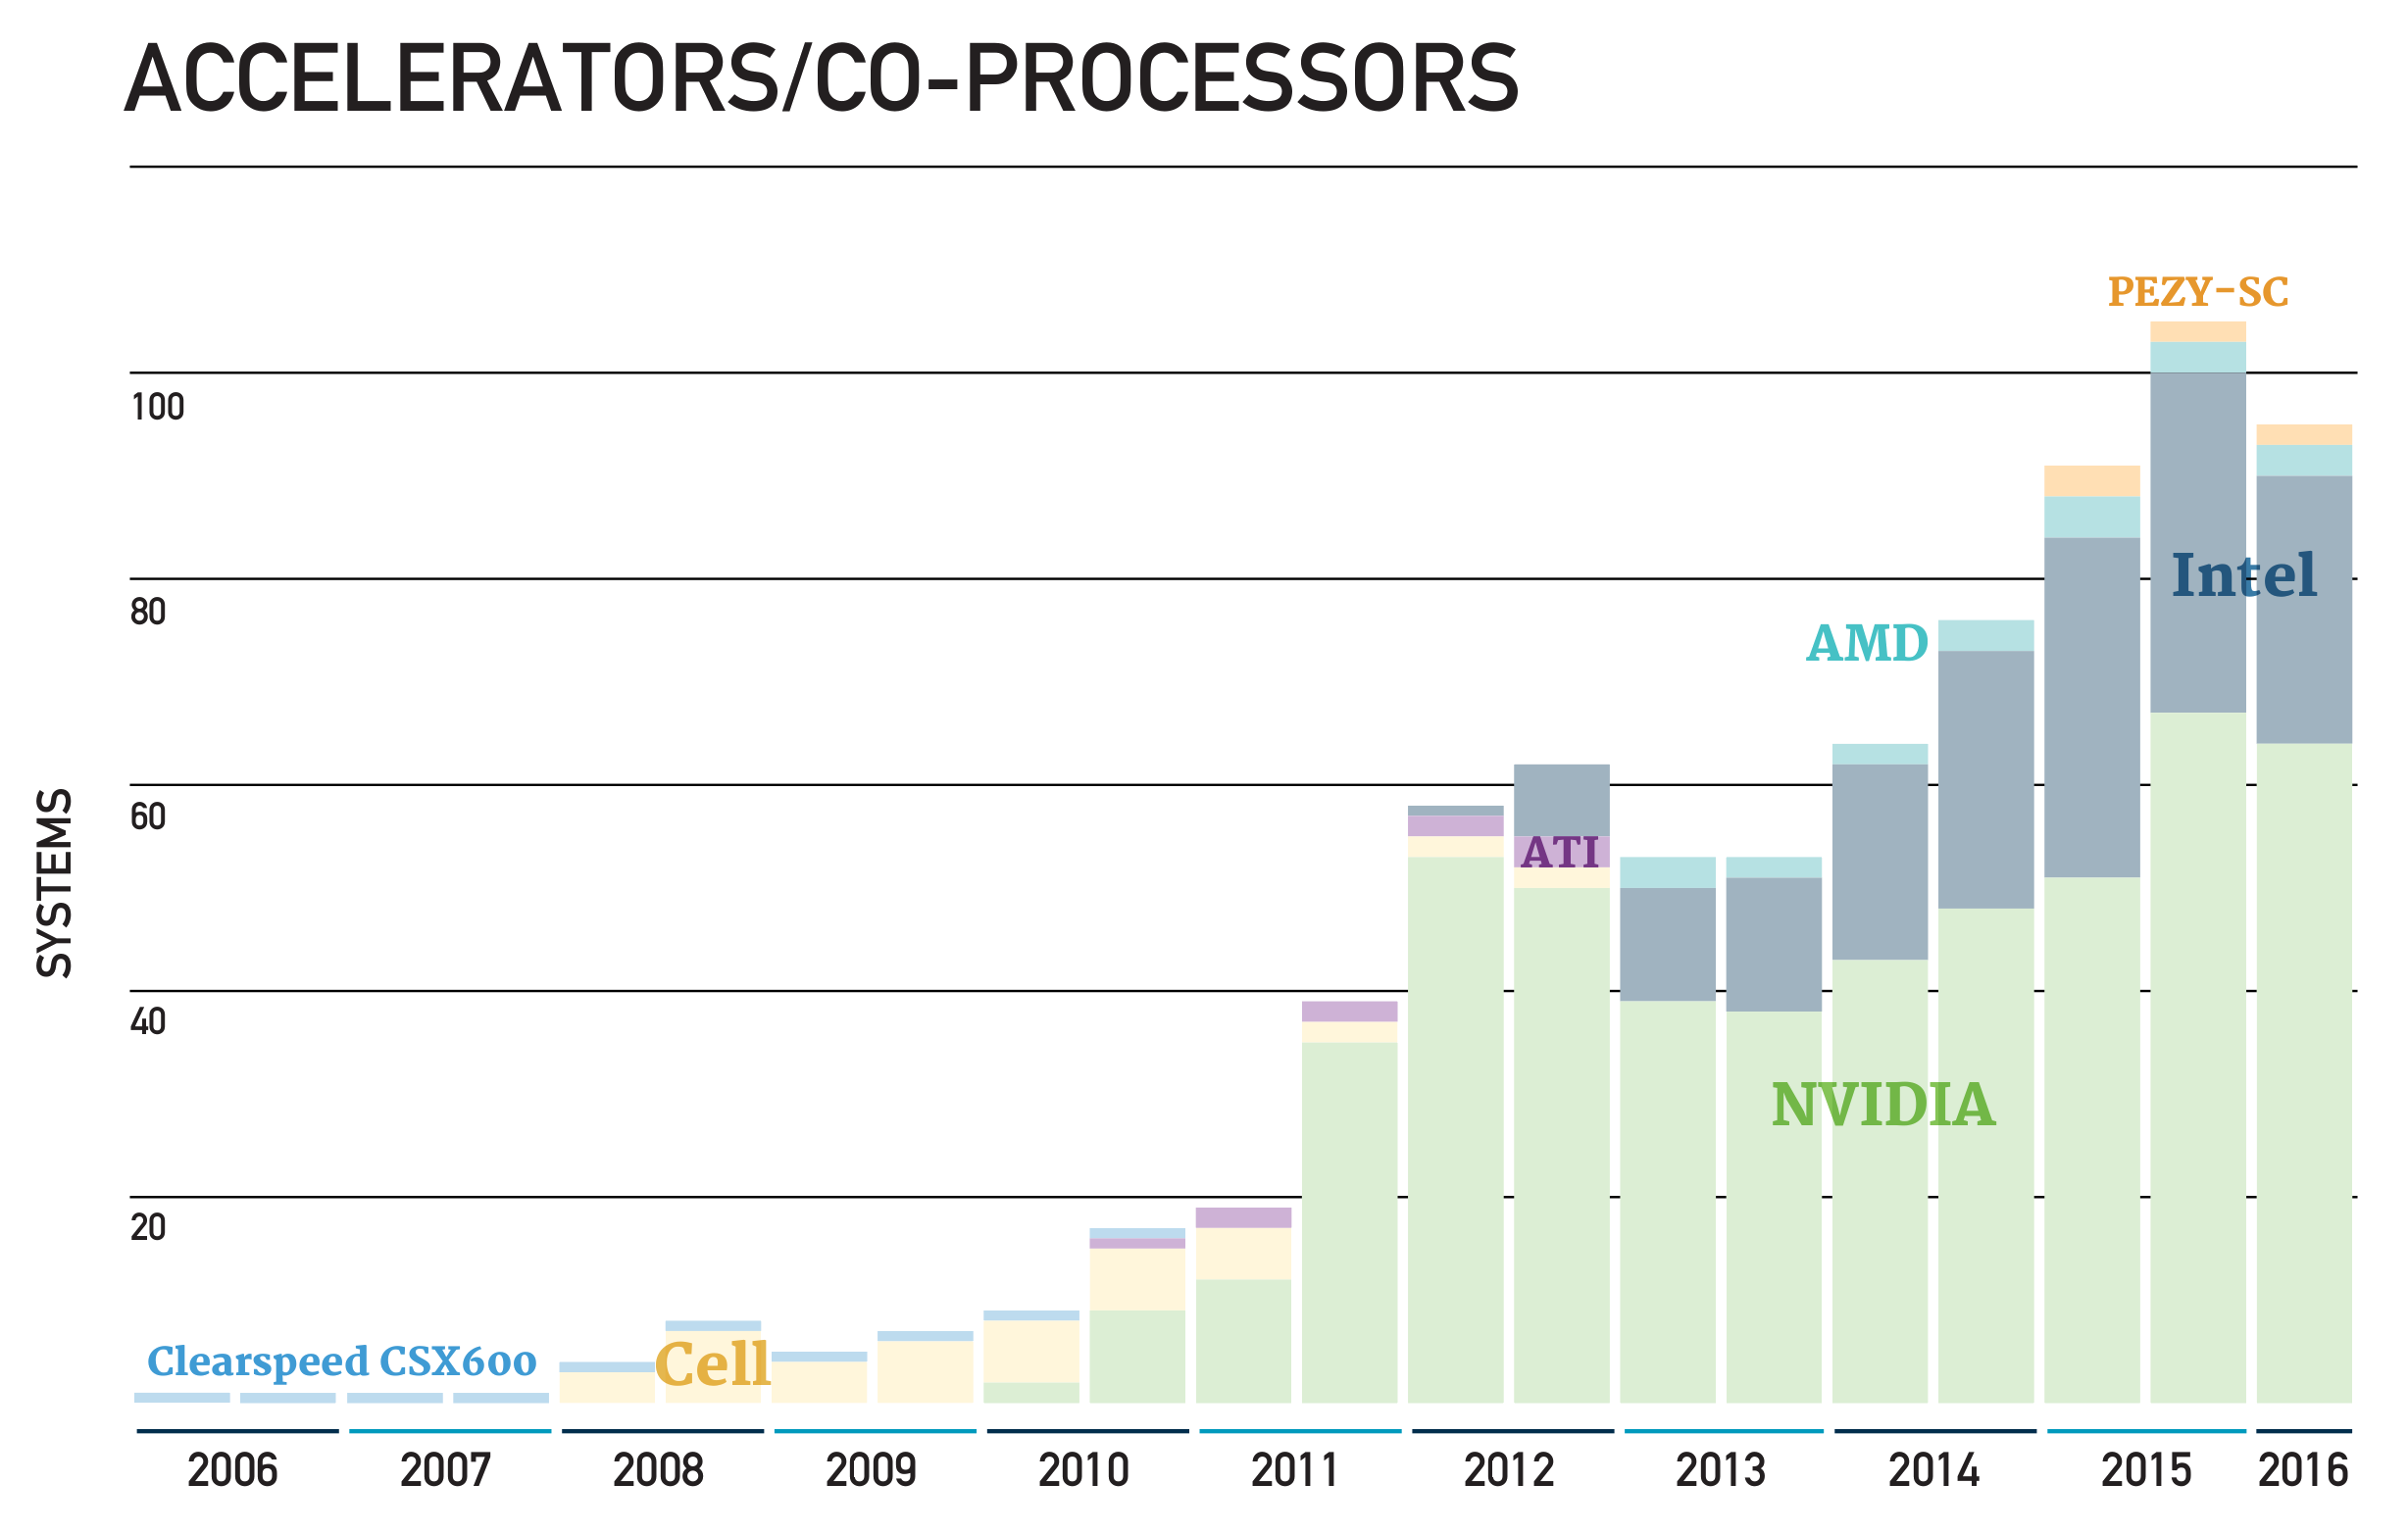
\includegraphics[width=.95\textwidth]{top500_accel}
    \hfill

        \tiny{Imagem: \url{top500.org/lists/2016/06/download/TOP500_201606_Poster.pdf} [Acessado em 29/07/16]}
    \end{center}
\end{frame}

\subsection{Computação Heterogênea}

\begin{frame}
    \frametitle{Computação Heterogênea}
    \begin{center}
        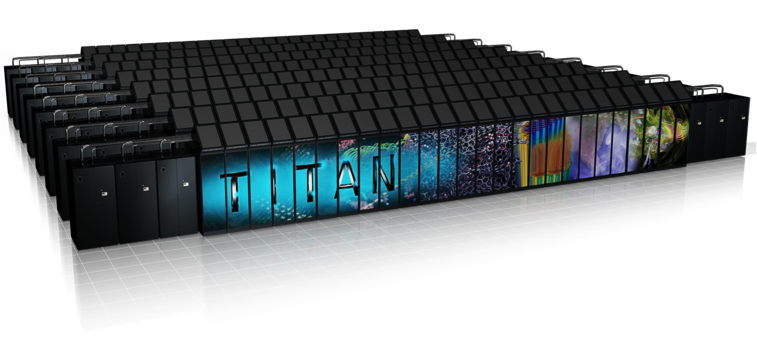
\includegraphics[width=.83\textwidth]{titan}
    \end{center}

    \pause

    Dados recursos computacionais \alert{heterogêneos}, conjuntos de
    \alert{dados} e \alert{computações}, como distribuir computações e dados de
    forma a \alert{otimizar o uso} dos recursos?
    \hfill

    \begin{center}
    \tiny{Imagem: \url{olcf.ornl.gov/titan} [Acessado em 29/07/16]}
    \end{center}
\end{frame}

\begin{frame}
    \frametitle{Computação Heterogênea}
    Recursos computacionais \alert{heterogêneos}:
    \pause
    \begin{itemize}
        \item Baixa latência: CPUs
            \pause
        \item Alta vazão: GPUs
            \pause
        \item Reconfiguráveis: FPGAs
            \pause
        \item Especializados: ASICs, DSPs
            \pause
        \item Memória?
    \end{itemize}
\end{frame}

\begin{frame}
    \frametitle{Computação Heterogênea}
    Conjuntos de \alert{dados}:
    \begin{itemize}
        \item \textit{Big Data}
        \item \textit{Data Streams}
        \item ...
    \end{itemize}
    \pause
    Modelos de programação (\alert{computações}):
    \begin{itemize}
        \item \textit{MapReduce}
        \item \textit{Task Parallelism}
        \item ...
    \end{itemize}
\end{frame}

\begin{frame}
    \frametitle{Computação Heterogênea: Escalabilidade}
    \begin{center}
        
\includegraphics[width=.7\textwidth]{scalability}
    \end{center}

    \alert{Escalabilidade} significa não perder desempenho
        executando em:
    \begin{itemize}
        \item Múltiplos \textit{cores} idênticos
            \pause
        \item Novas versões do mesmo \textit{core}
    \end{itemize}
\end{frame}

\begin{frame}
    \frametitle{Computação Heterogênea: Portabilidade}
    \begin{center}
        
\includegraphics[width=.7\textwidth]{portability}
    \end{center}

    \alert{Portabilidade} significa não perder desempenho
        executando em diferentes:
    \begin{itemize}
        \item \textit{Cores} ou \alert{aceleradores}
            \pause
        \item Modelos de memória
            \pause
        \item Modelos de paralelismo
            \pause
        \item Conjuntos de instruções
    \end{itemize}
\end{frame}

\begin{frame}
    \frametitle{Computação Heterogênea}
    \centering
    
\includegraphics[width=.85\textwidth]{heterogeneous}
\end{frame}

\begin{frame}
    \frametitle{Computação Heterogênea}
    \centering
    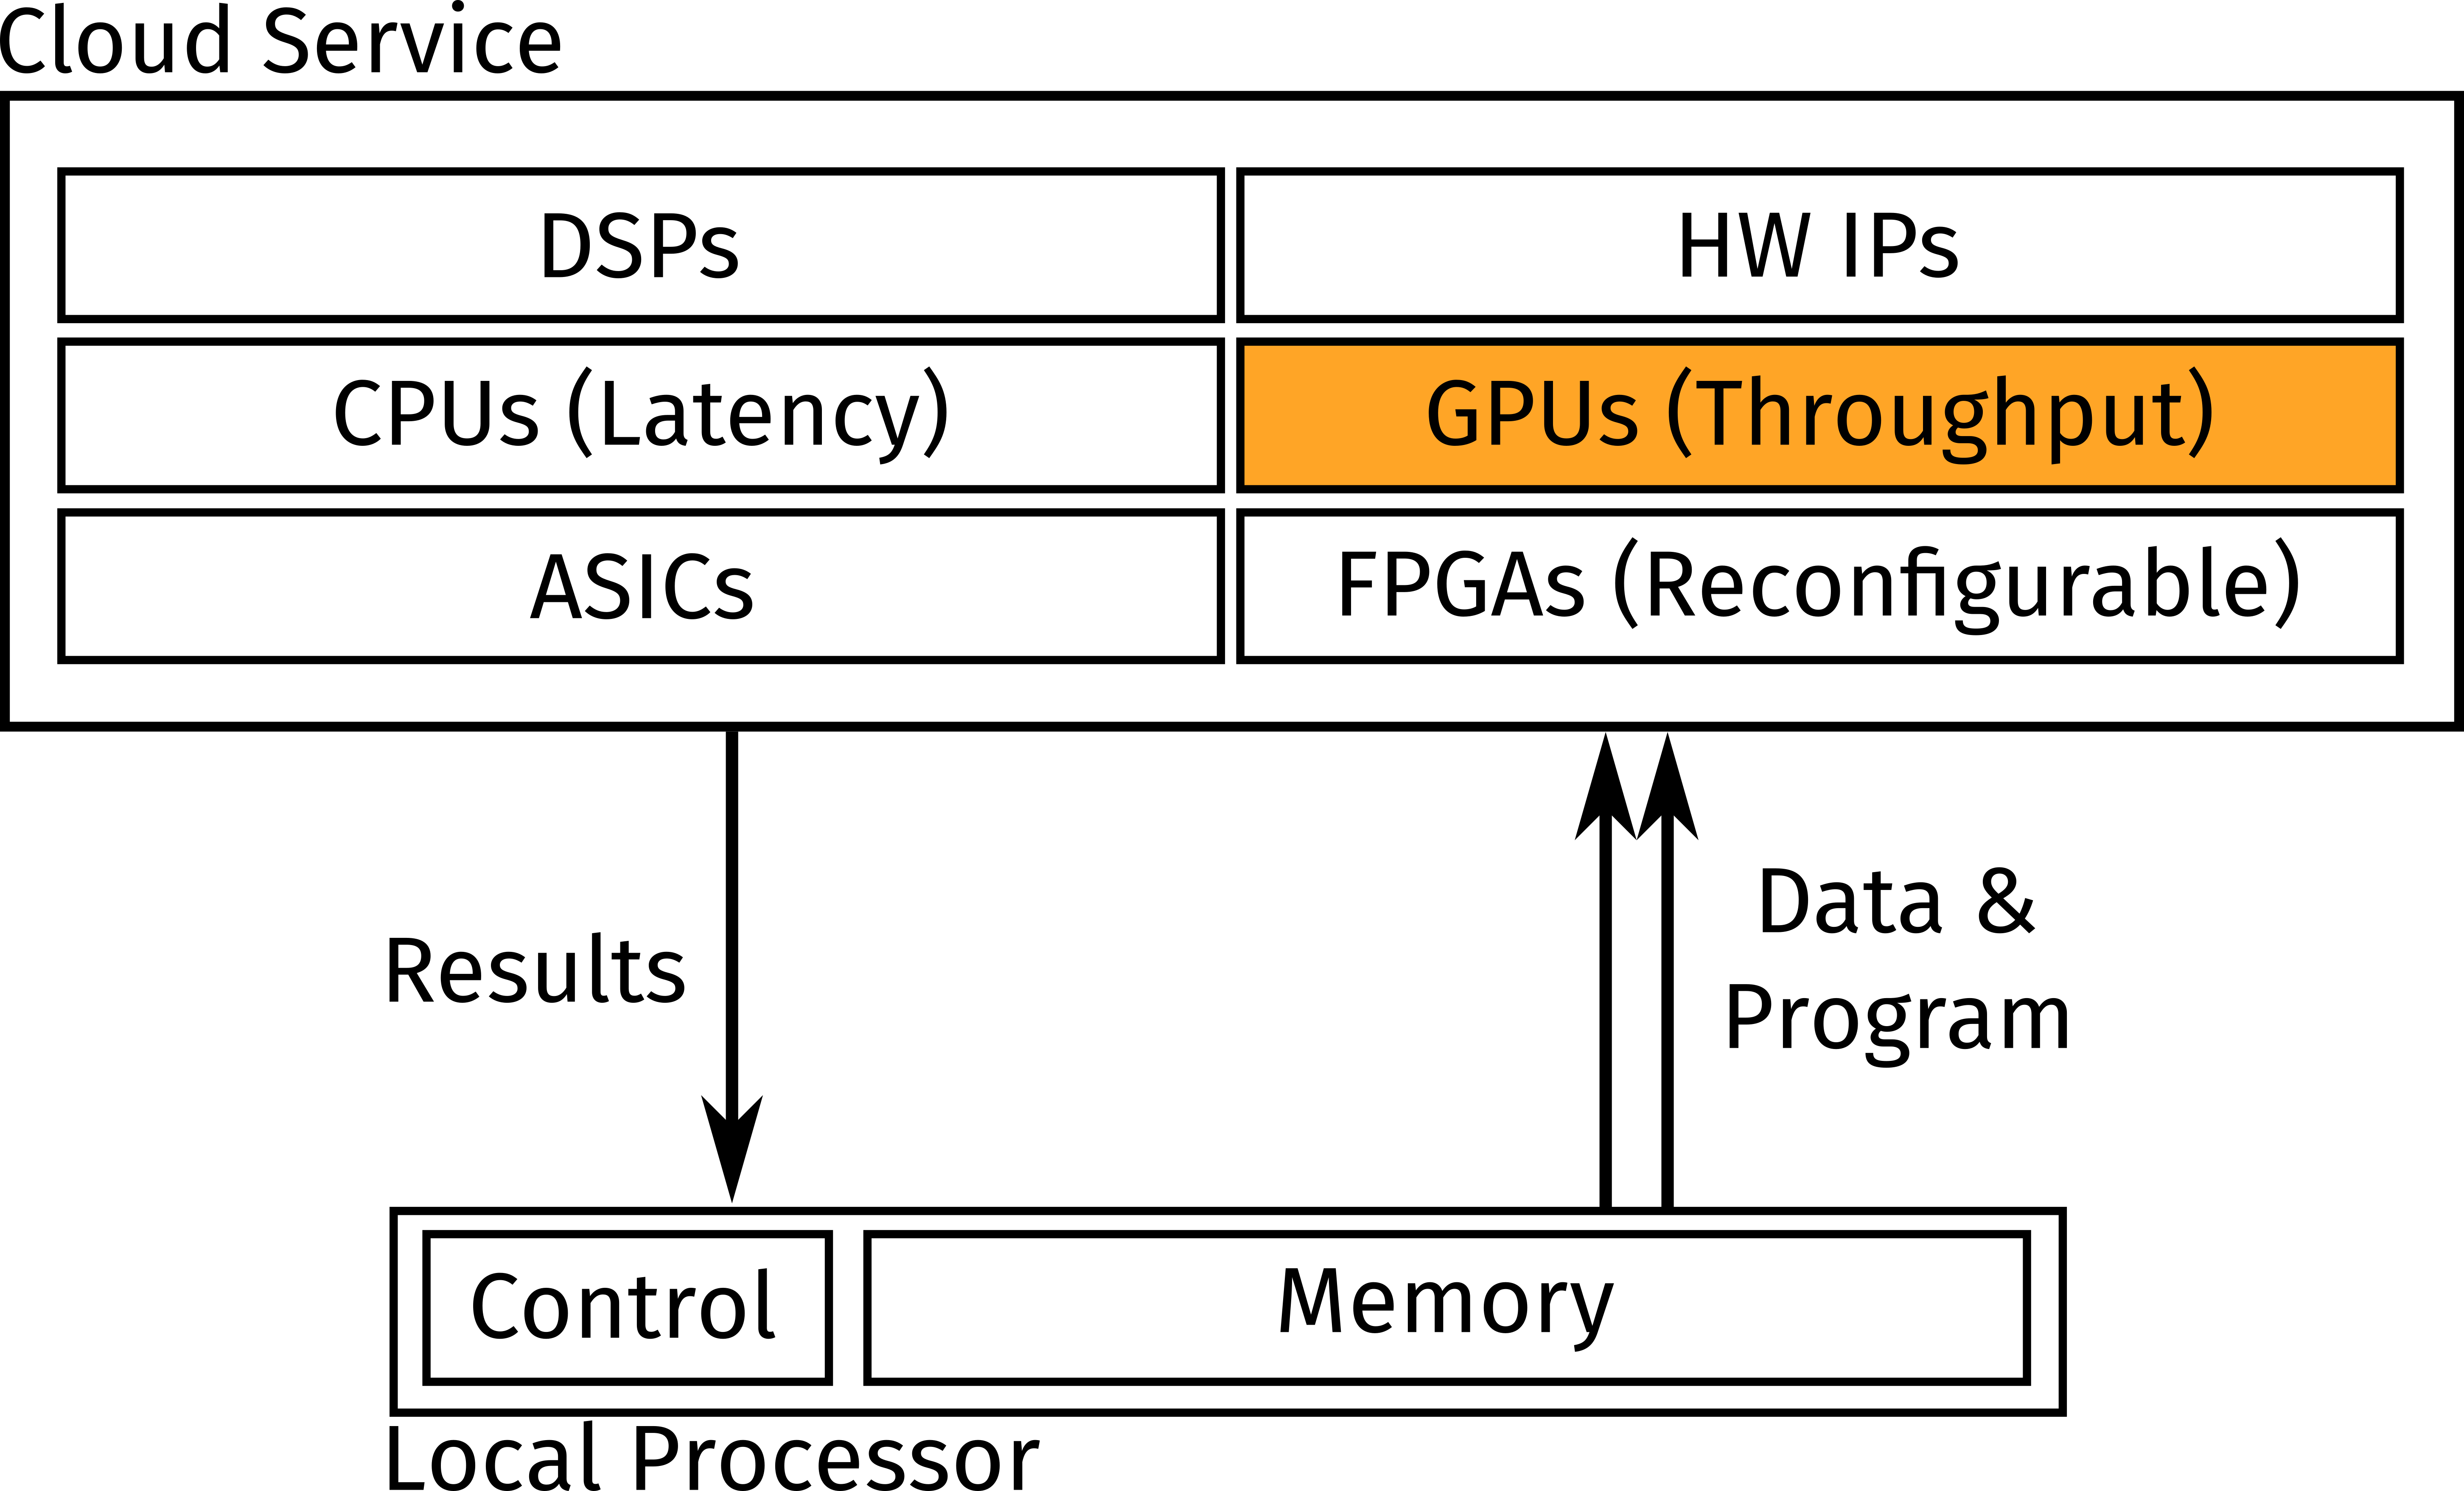
\includegraphics[width=.85\textwidth]{heterogeneous_highlight}
\end{frame}

\section{GPUs}

\begin{frame}
    \frametitle{Graphics Processing Units}
    \begin{center}
        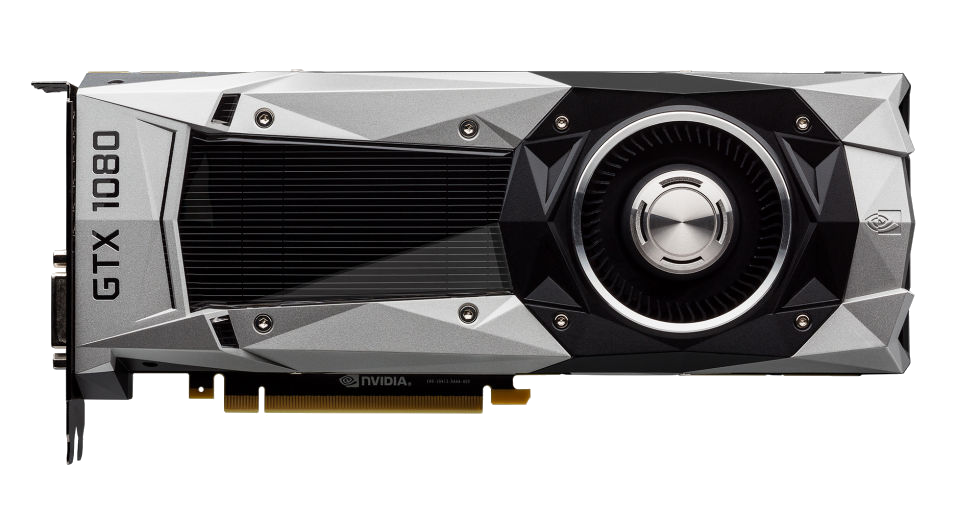
\includegraphics[width=.6\textwidth]{gtx1080}
    \end{center}
    \pause

    Originalmente especializadas em \alert{processamento gráfico},
    trabalham com muitos dados e têm \alert{alta vazão}:
    \pause

    \begin{itemize}
        \item Caches pequenos (\textit{kilobytes})
            \pause
        \item Sem \alert{branch prediction}
            \pause
        \item \alert{Milhares} de ALUs de \alert{maior latência}
            \pause
        \item \alert{Pipelines} de execução
            \pause
        \item 114 688 \alert{threads} concorrentes na arquitetura Pascal
    \end{itemize}
\end{frame}

\begin{frame}
    \frametitle{Graphics Processing Units}
    Hoje são usadas em computação de propósito geral, podem ser chamadas de
    \textit{General Purpose GPUs} (GPGPUs):
    \pause
    \begin{itemize}
        \item \textit{OpenGL}: 1992
        \item \textit{DirectX}: 1995
        \item \alert{CUDA}: 2007
        \item \textit{OpenCL}: 2009
        \item \textit{Vulkan}: 2016
    \end{itemize}
\end{frame}

\subsection{Modelo de Hardware}

\begin{frame}
    \frametitle{Modelo de \textit{Hardware}}
    Taxonomia de Flynn:
    \begin{itemize}
        \item \textit{Single Instruction Multiple Data} (SIMD)
            \pause
        \item \textit{Single Instruction Multiple Thread} (SIMT)?
    \end{itemize}
    \pause
    Escalonamento e execução:
    \begin{itemize}
        \item \textit{Streaming Multiprocessor} (SM)
            \pause
        \item \textit{Warps}
            \pause
        \item \textit{Grids, blocks} e \textit{threads}
    \end{itemize}
\end{frame}

\begin{frame}
    \frametitle{Modelo de \textit{Hardware}}
    Escalonamento de mais alto-nível:
    \begin{itemize}
        \item \textit{Pipelines}
        \item \textit{Texture Processing Cluster} (TPC)
        \item \textit{Graphics Processing Cluster} (GPC)
    \end{itemize}
    \pause
    Memória:
    \begin{itemize}
        \item Compartilhada: Cache L1, L2; \textit{megabytes} (Nvidia Pascal)
        \item Global: volátil, GDDR5; \textit{gigabytes}
            \pause
        \item SSD: \alert{não-volátil}; \alert{\textit{terabytes}} (AMD SSG Fiji, 2017)
    \end{itemize}
    \vfill

    \tiny{AMD SSG: \url{anandtech.com/show/10518/amd-announces-radeon-pro-ssg-fiji-with-m2-ssds-onboard} [Acessado em 30/07/16]}
\end{frame}

\subsection{Compute Capability e SIMT}

\begin{frame}
    \frametitle{\textit{Compute Capability} e SIMT}
    A \alert{Compute Capability} especifica características de
    arquiteturas \textit{Single Instruction Multiple Thread} (SIMT):
    \pause
    \begin{itemize}
        \item \textit{Warp}: Grupo de \textit{threads} executadas em \alert{paralelo}
        \item \textit{Streaming Multiprocessor} (SM): Cria, escalona e executa \textit{warps}
            \pause
        \item Múltiplas \textit{warps} \alert{concorrentes} no mesmo SM
    \end{itemize}
    \vfill

    \begin{center}
        \tiny{Fonte: \url{docs.nvidia.com/cuda/cuda-c-programming-guide/index.html\#hardware-implementation} [Acessado em 29/07/16]}
    \end{center}
\end{frame}

\begin{frame}
    \frametitle{\textit{Compute Capability} e SIMT}
    \textit{Warps}:
    \pause
    \begin{itemize}
        \item Unidade de execução e escalonamento
        \item 32 \textit{threads}
            \pause
        \item 1 \alert{instrução em comum} por vez
            \pause
        \item \textit{Threads ativas}: estão no \textit{branch} atual de
            execução
        \item \textit{Threads inativas}: \alert{não} estão no \textit{branch}
            atual de execução
            \pause
        \item \textit{Threads} fora do \textit{branch} atual executadas
            \alert{sequencialmente}
            \pause
        \item Eficiência: sem divergência de execução dentro de \textit{Warps}
    \end{itemize}
    \vfill

    \begin{center}
        \tiny{Fonte: \url{docs.nvidia.com/cuda/cuda-c-programming-guide/index.html\#hardware-implementation} [Acessado em 29/07/16]}
    \end{center}
\end{frame}

\subsection{Arquitetura Pascal GP100}

\begin{frame}
    \frametitle{Arquitetura Pascal GP100}
    \centering
    \includegraphics[width=.65\textwidth]{gp100_view}
    \vfill

    \tiny{Imagem: \url{images.nvidia.com/content/pdf/tesla/whitepaper/pascal-architecture-whitepaper.pdf} [Acessado em 29/07/16]}
\end{frame}

\begin{frame}
    \frametitle{Arquitetura Pascal GP100: \textit{Compute Capability 6.0}}
    \centering
    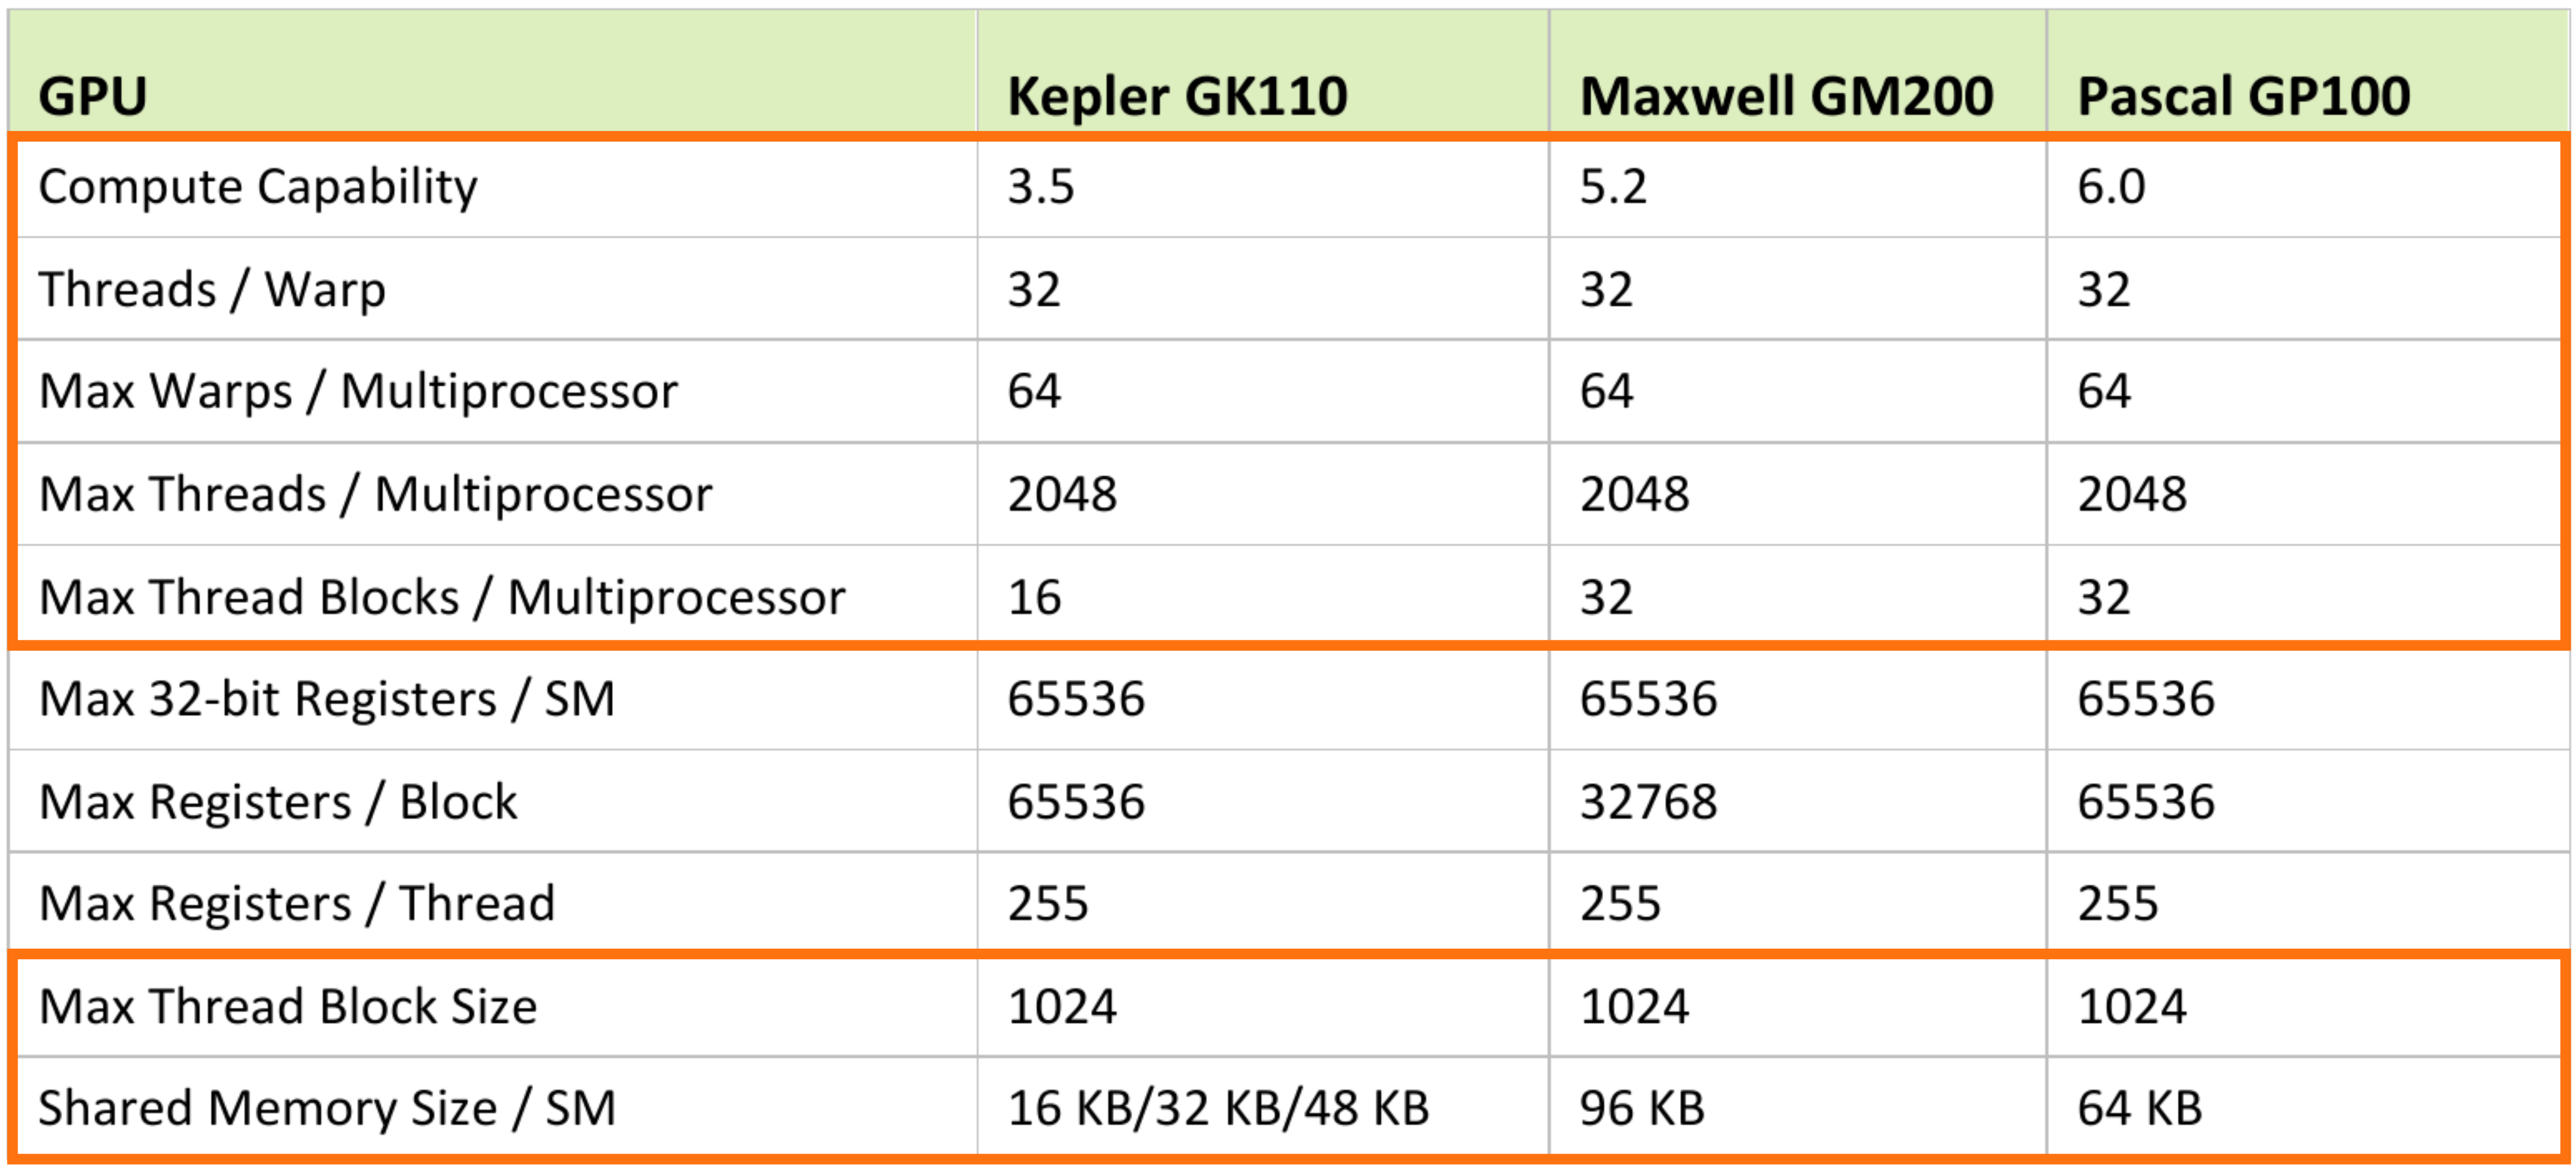
\includegraphics[width=\textwidth]{cc_6_highlight}
    \vfill

    \tiny{Imagem: \url{images.nvidia.com/content/pdf/tesla/whitepaper/pascal-architecture-whitepaper.pdf} [Acessado em 29/07/16]}
\end{frame}

\begin{frame}
    \frametitle{Arquitetura Pascal GP100: SM}
    \centering
    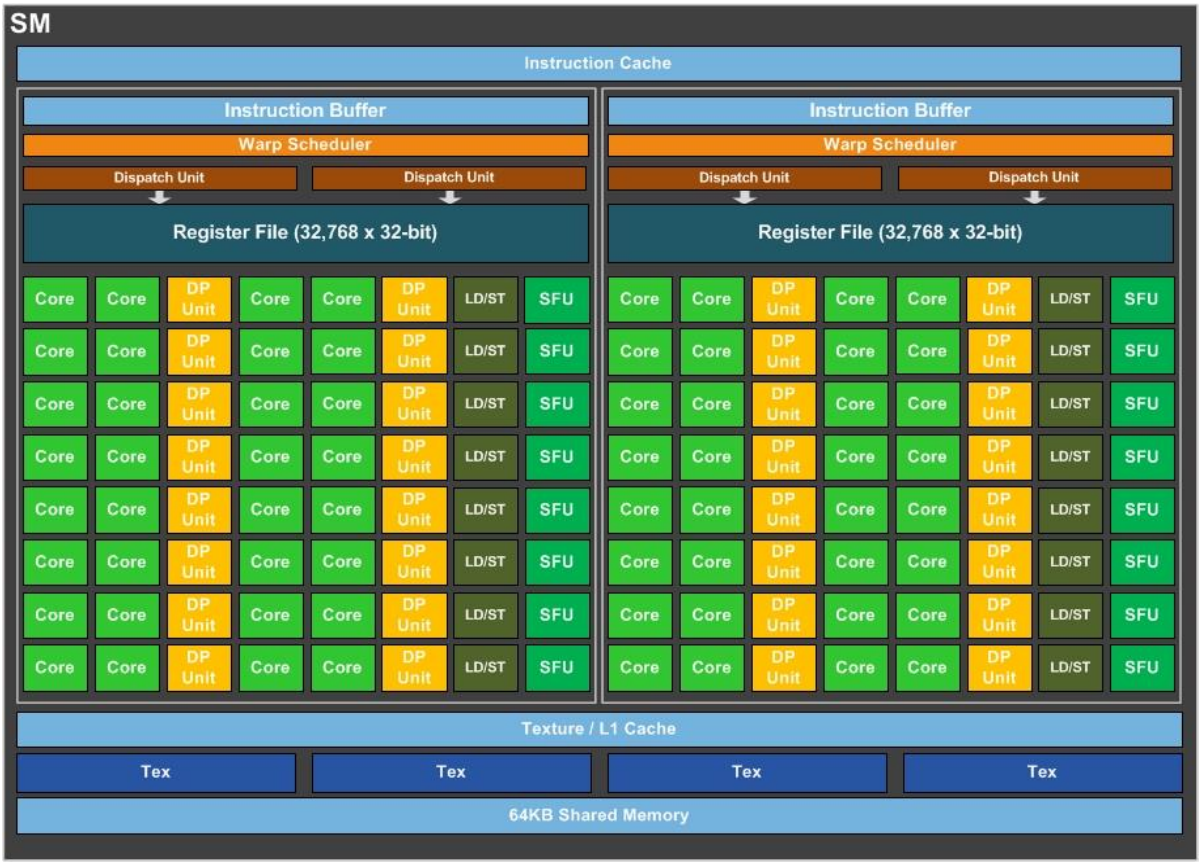
\includegraphics[width=.9\textwidth]{gp100_SM_diagram}
    \vfill

    \tiny{Imagem: \url{images.nvidia.com/content/pdf/tesla/whitepaper/pascal-architecture-whitepaper.pdf} [Acessado em 29/07/16]}
\end{frame}

\begin{frame}
    \frametitle{Arquitetura Pascal GP100}
    \centering
    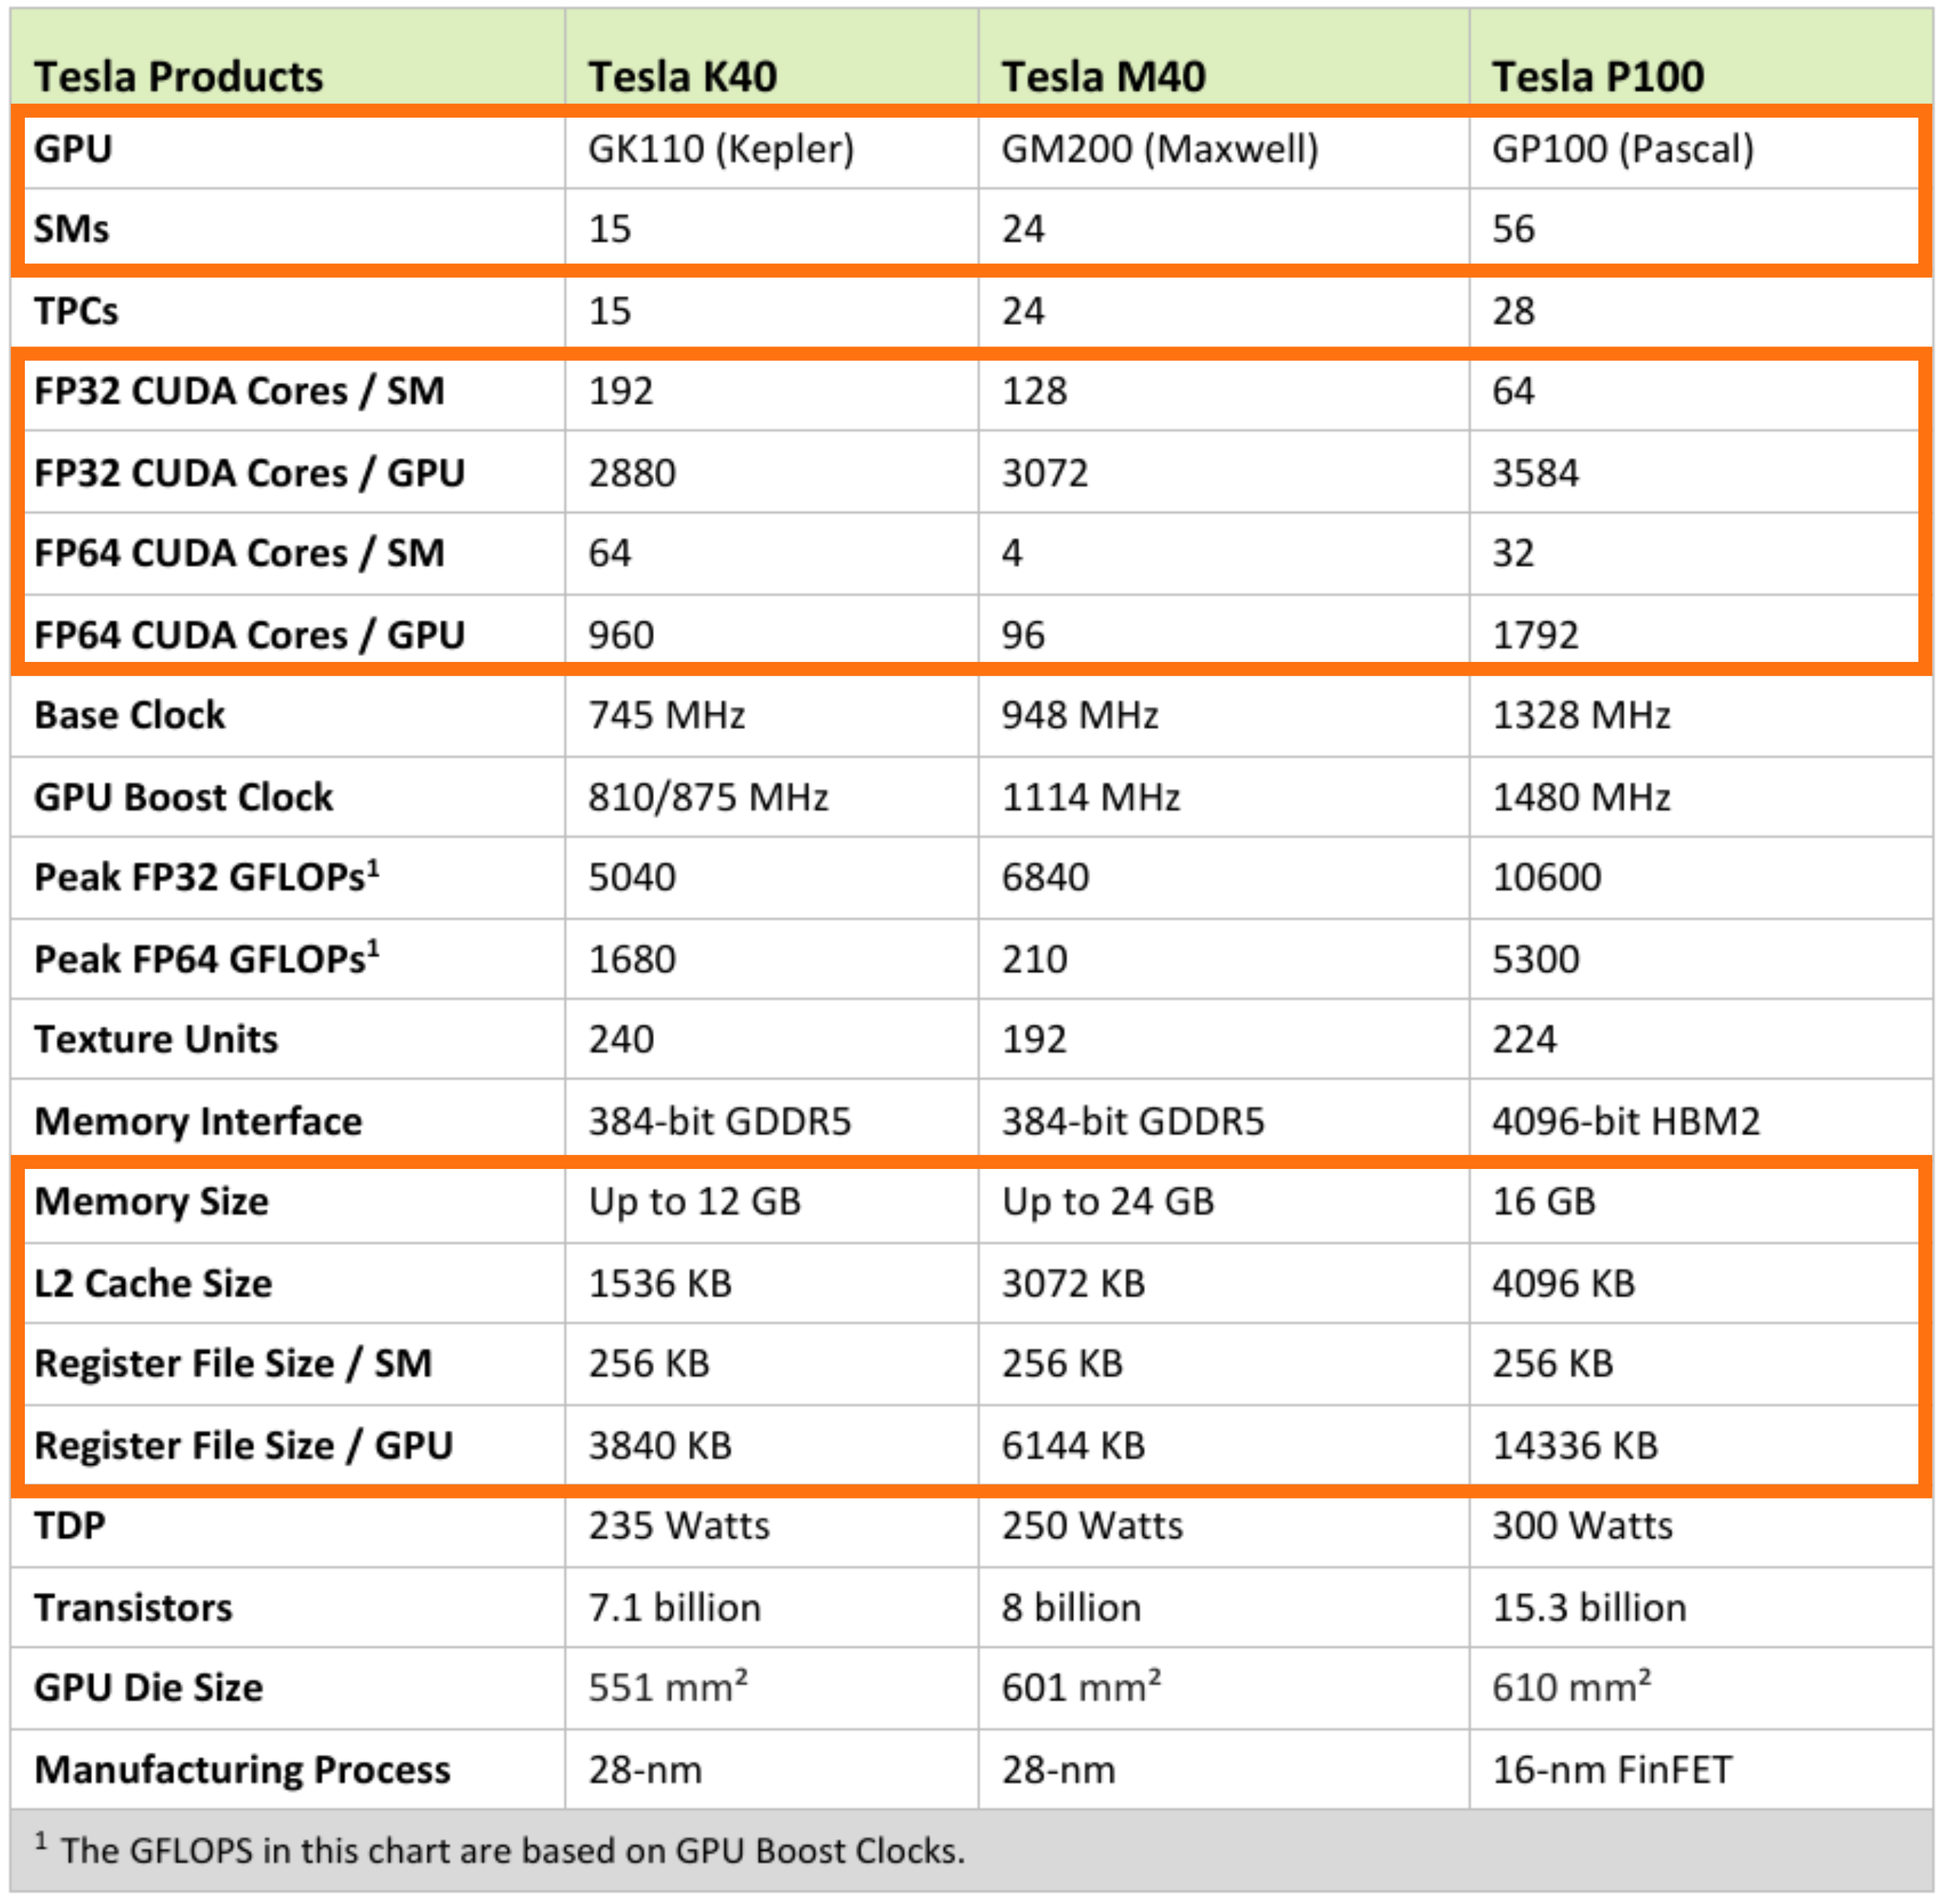
\includegraphics[width=.7\textwidth]{gp100_stats_highlight}
    \vfill

    \tiny{Imagem: \url{images.nvidia.com/content/pdf/tesla/whitepaper/pascal-architecture-whitepaper.pdf} [Acessado em 29/07/16]}
\end{frame}

\begin{frame}
    \frametitle{Arquitetura Pascal GP100}
    \centering
    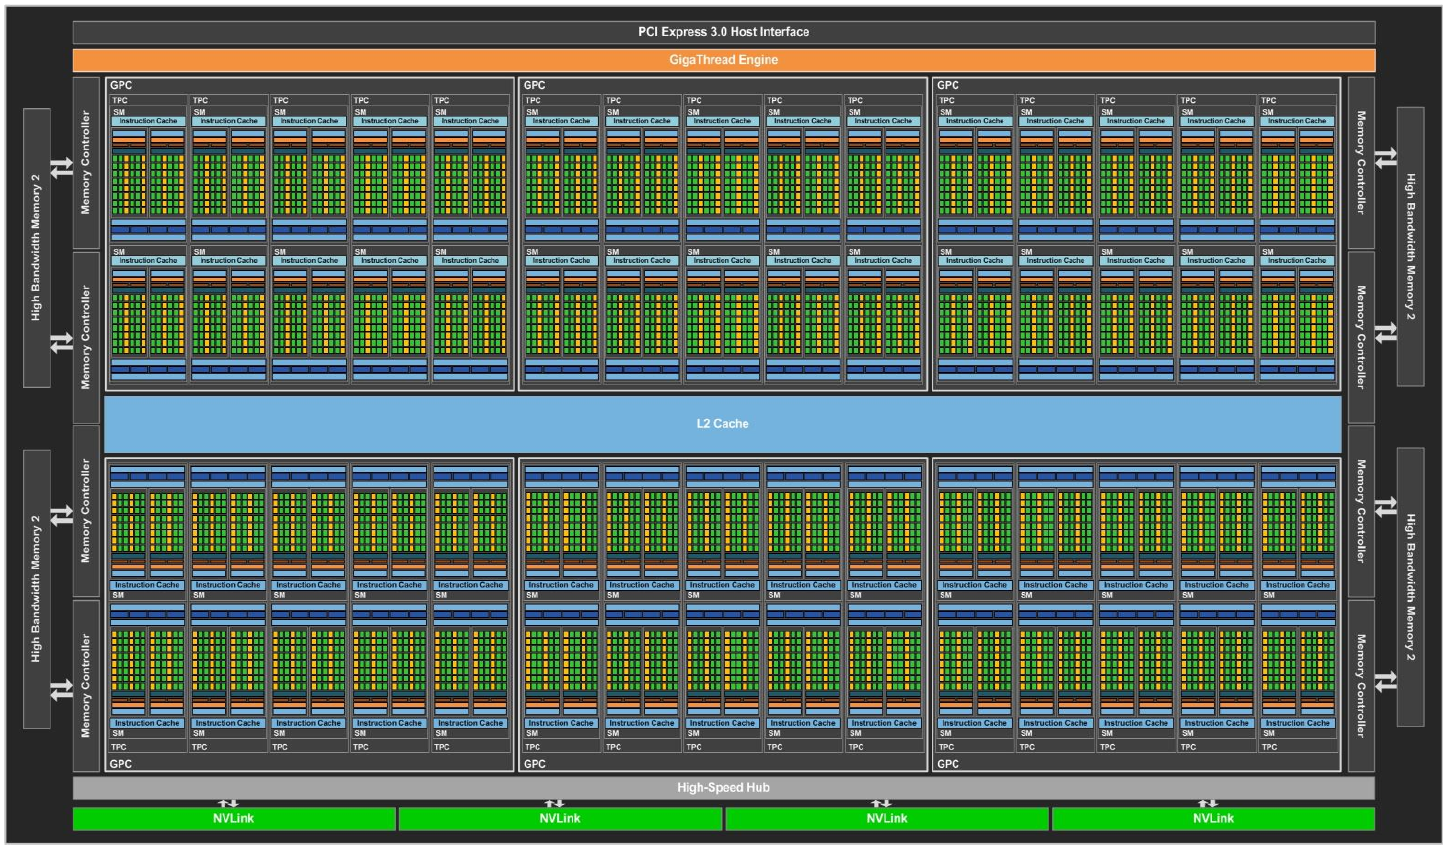
\includegraphics[width=.95\textwidth]{gp100_diagram}
    \vfill

    \tiny{Imagem: \url{images.nvidia.com/content/pdf/tesla/whitepaper/pascal-architecture-whitepaper.pdf} [Acessado em 29/07/16]}
\end{frame}

\section{Plataforma CUDA}

\begin{frame}
    \frametitle{Plataforma CUDA}
    \begin{center}
        
\includegraphics[width=.4\textwidth]{cuda-logo}
    \end{center}
    \pause

    \begin{itemize}
        \item Plataforma para \alert{computação paralela}
        \item \textit{Application Programming Interface} (API)
        \item CUDA \textit{Toolkit}
    \end{itemize}
\end{frame}

\subsection{Aceleração por Software}

\begin{frame}
    \frametitle{Aceleração por \textit{Software}}
    \centering
    
\includegraphics[width=.95\textwidth]{accel_apps}
\end{frame}

\subsection{Bibliotecas}

\begin{frame}
    \frametitle{Bibliotecas}
    \begin{center}
        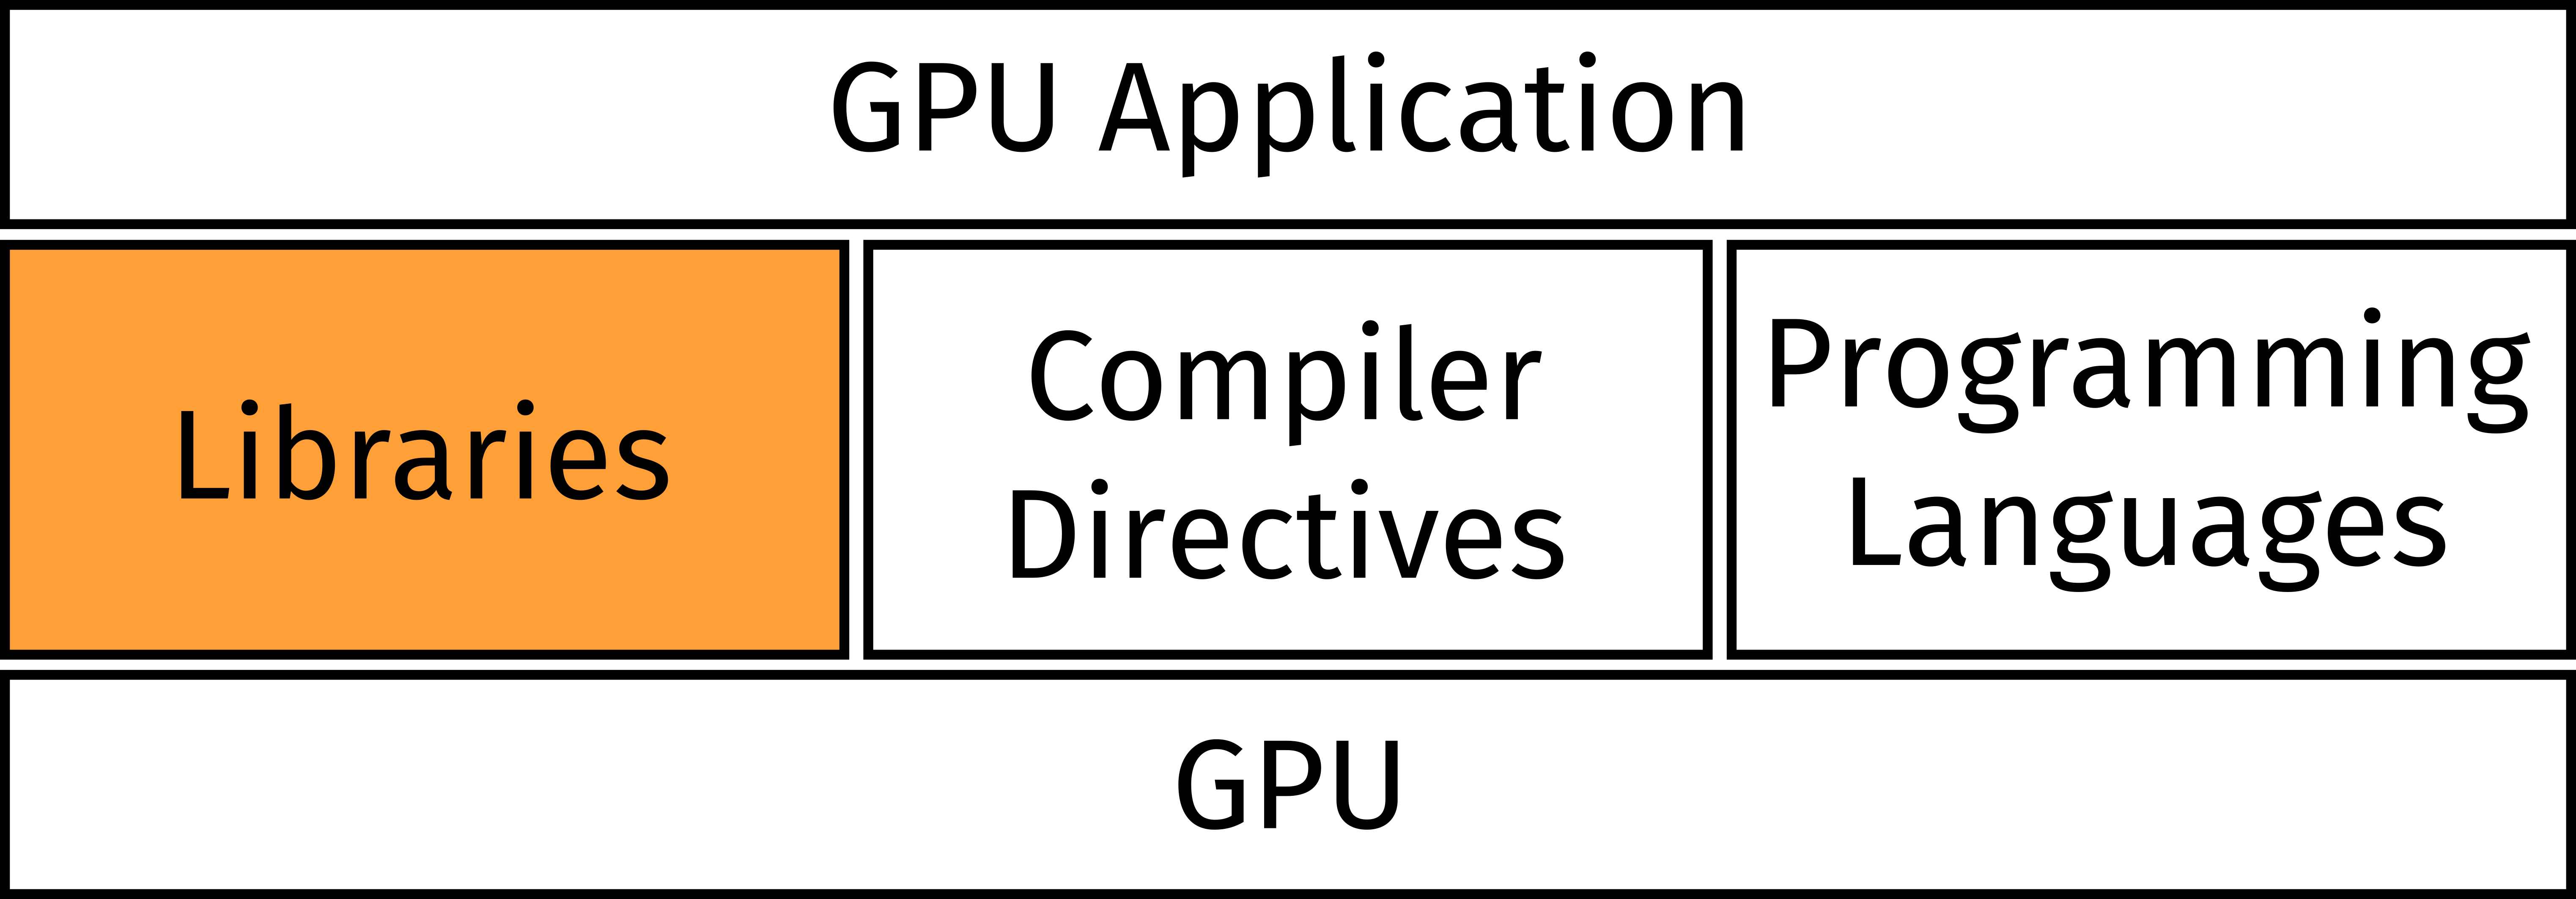
\includegraphics[width=.6\textwidth]{accel_apps_lib}
    \end{center}
    \pause

    \begin{itemize}
        \item Fáceis de usar
            \pause
        \item Aceleração \textit{Drop-in}
            \pause
        \item Otimizadas por especialistas
    \end{itemize}
\end{frame}

\begin{frame}
    \frametitle{Bibliotecas}
    \centering
    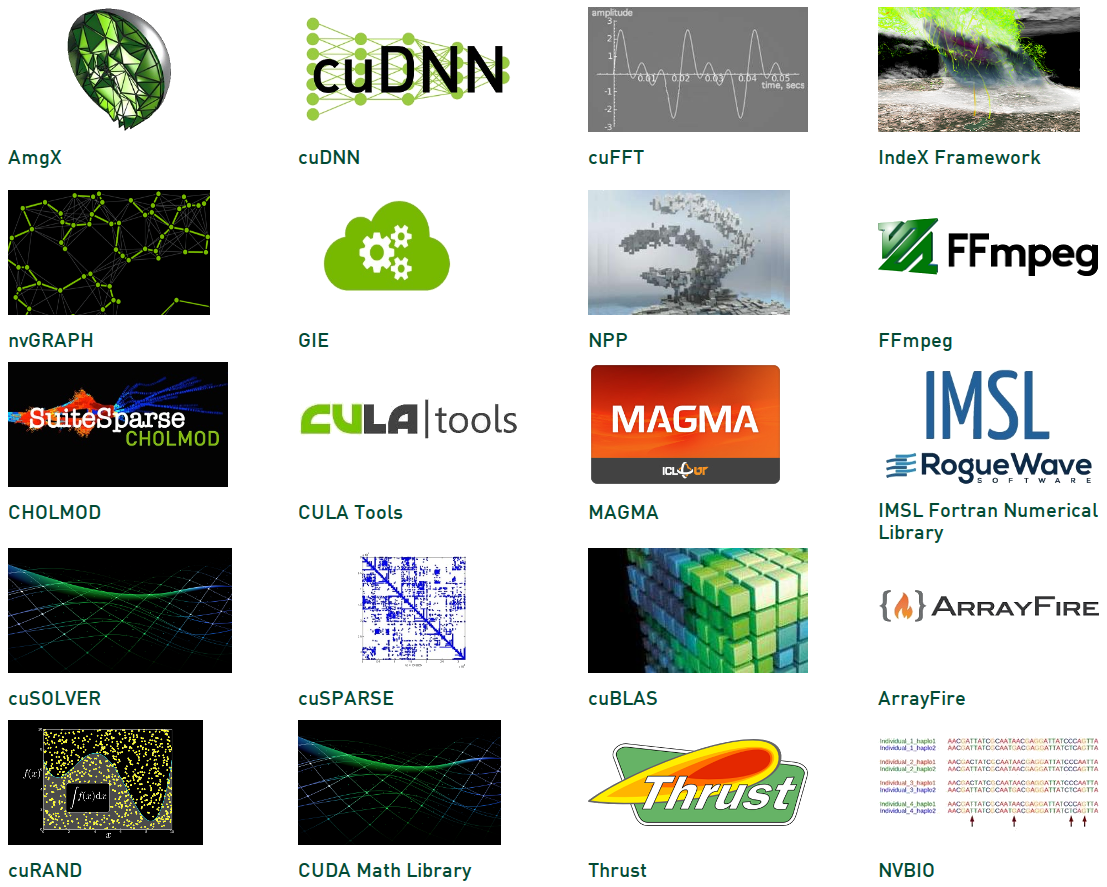
\includegraphics[width=.9\textwidth]{accel_libs_no}
    \vfill

    \tiny{Imagem: \url{developer.nvidia.com/gpu-accelerated-libraries} [Acessado em 29/07/16]}
\end{frame}

\begin{frame}[fragile]
    \frametitle{Bibliotecas}
    Soma de vetores com a biblioteca \alert{Thrust}:
    \begin{lstlisting}
    thrust::device_vector<float> device_input1(input_lenght);
    thrust::device_vector<float> device_input2(input_lenght);
    thrust::device_vector<float> device_output(input_lenght);
    \end{lstlisting}
    \pause
    \begin{lstlisting}
    thrust::copy(host_input1, host_input1 + input_lenght, device_input1.begin());

    thrust::copy(host_input2, host_input2 + input_lenght, device_input2.begin());
    \end{lstlisting}
    \pause
    \begin{lstlisting}
    thrust::transform(device_input1.begin(), device_input1.end(), device_input2.begin(), device_output.begin(), thrust::plus<float>());
    \end{lstlisting}
\end{frame}

\subsection{Diretivas de Compilação}

\begin{frame}
    \frametitle{Diretivas de Compilação}
    \begin{center}
        
\includegraphics[width=.6\textwidth]{accel_apps_comp}
    \end{center}
    \pause

    \begin{itemize}
        \item Fáceis de usar
            \pause
        \item Portáveis, mas desempenho depende do compilador
    \end{itemize}
\end{frame}

\begin{frame}[fragile]
    \frametitle{Diretivas de Compilação}
    Soma de vetores com \alert{OpenACC}:
    \begin{lstlisting}
    #pragma acc data copyin(input1[0:input_lenght],input2[0:input_lenght]), copyout(output[0:input_lenght])
    \end{lstlisting}
    \pause
    \begin{lstlisting}
    {
        #pragma acc kernels loop independent
        for(i = 0; i < input_lenght; i++) {
            output[i] = input1[i] + input2[i];
        }
    }
    \end{lstlisting}
\end{frame}

\subsection{Linguagens de Programação}

\begin{frame}
    \frametitle{Linguagens de Programação}
    \begin{center}
        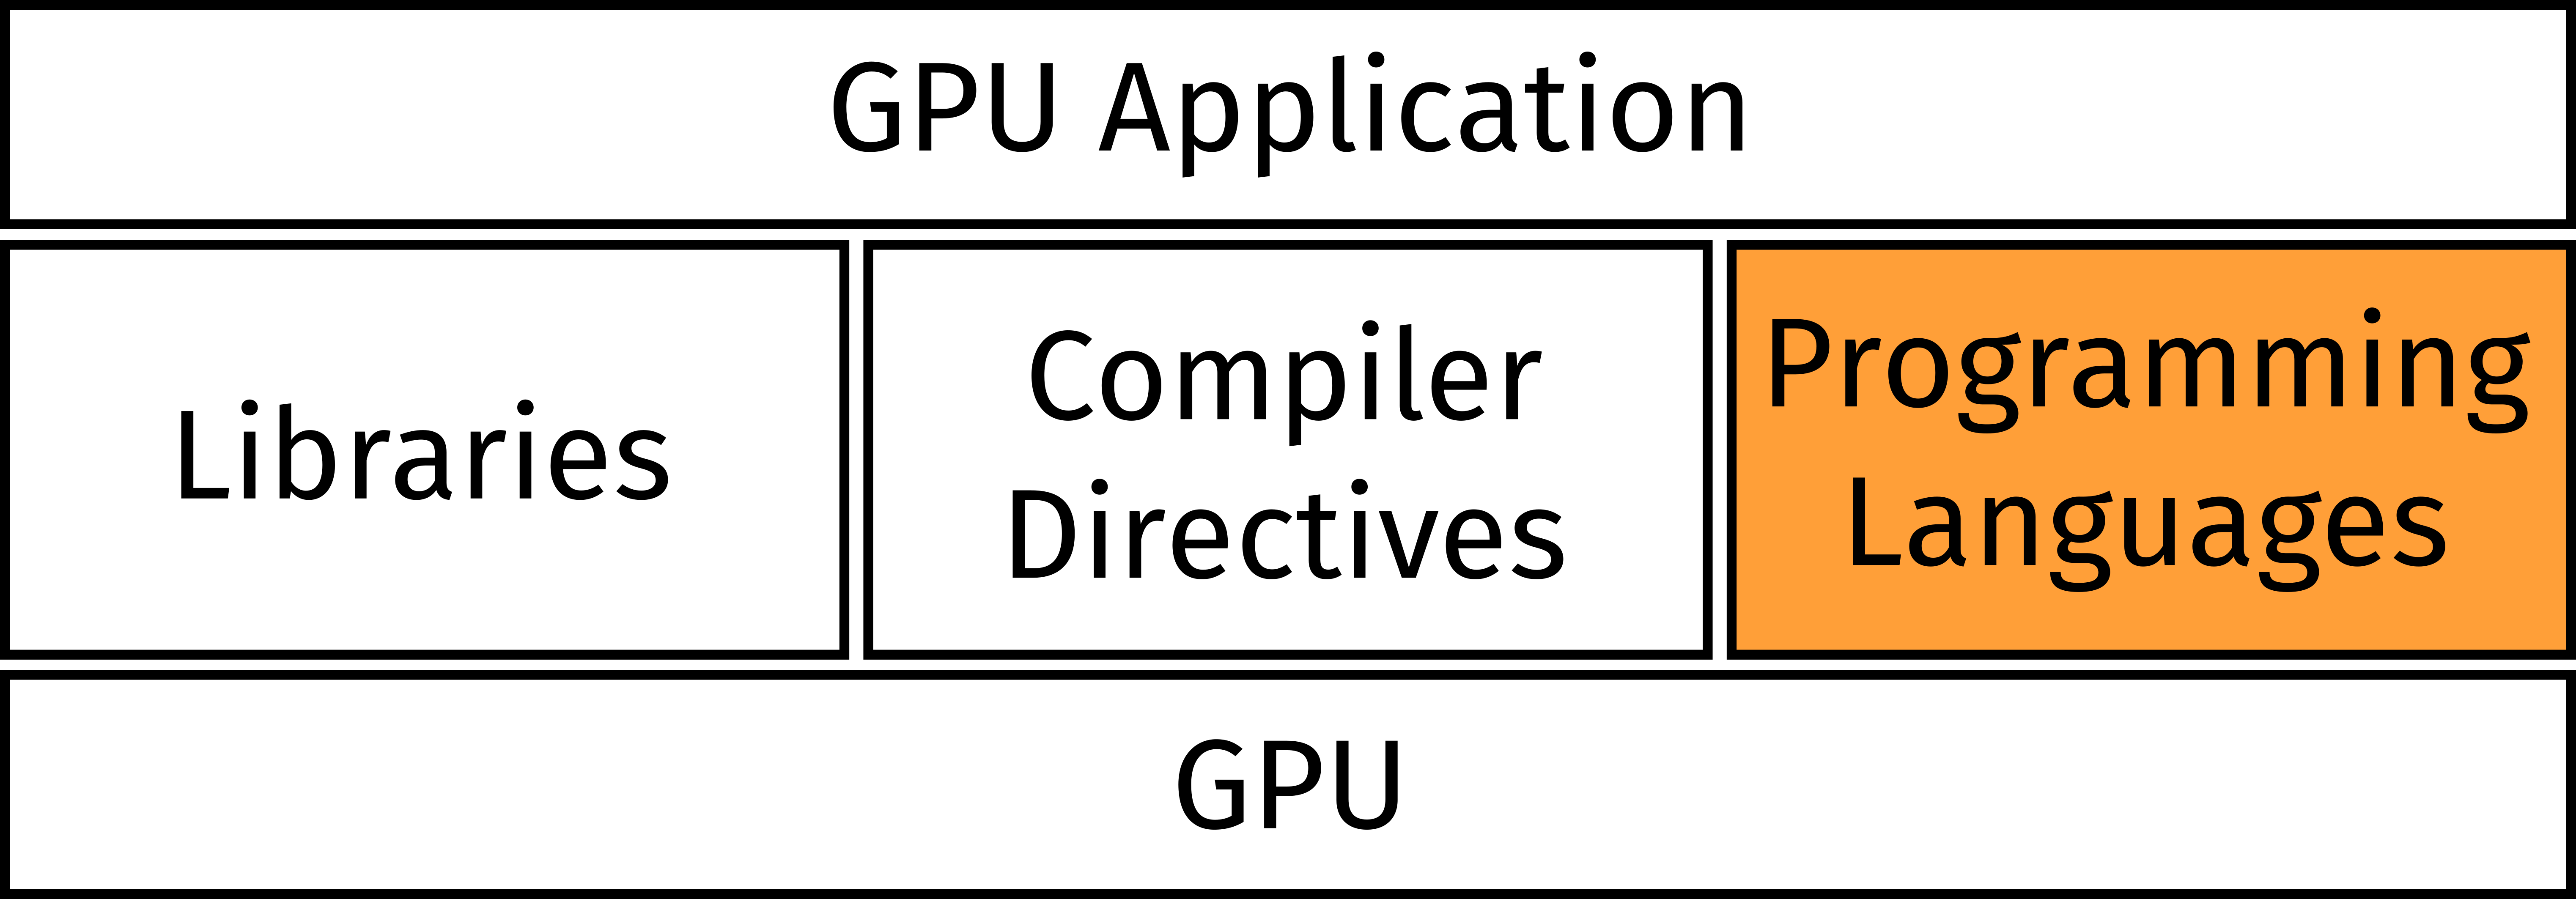
\includegraphics[width=.6\textwidth]{accel_apps_lang}
    \end{center}
    \pause

    \begin{itemize}
        \item Melhor desempenho, mas mais difíceis de usar
            \pause
        \item Flexíveis
    \end{itemize}
\end{frame}

\begin{frame}
    \frametitle{Linguagens de Programação}
    Implementações de CUDA em:
    \begin{itemize}
        \item \alert{C}
        \item Fortran
        \item C++
        \item Python
        \item F\#
    \end{itemize}
\end{frame}

\section{CUDA C}

\begin{frame}
    \frametitle{CUDA C}
    \begin{center}
        
\includegraphics[width=.3\textwidth]{cuda-c}
    \end{center}

    \pause
    Modelo de Programação:
    \pause
    \begin{itemize}
        \item \alert{Kernels}
            \pause
        \item Hierarquia de \alert{Threads}
            \pause
        \item Hierarquia de \alert{Memória}
            \pause
        \item Programação \alert{Heterogênea}
    \end{itemize}
\end{frame}

\subsection{Kernel}

\begin{frame}
    \frametitle{CUDA C: \textit{Kernel}}
    \alert{Kernels}:
    \begin{itemize}
        \item \alert{Kernels} são funções C executadas por \alert{threads}
        \item $N$ \textit{threads} executam $N$ \textit{kernels}
            \pause
        \item Acessam \alert{ID} de suas \textit{threads} pela variável \alert{\texttt{threadIdx}}
            \pause
        \item Definidos usando a palavra-chave \alert{\texttt{\_\_global\_\_}}
        \item Seu tipo deve ser \alert{\texttt{void}}
    \end{itemize}

    \vfill

    \begin{center}
        \tiny{Fonte: \url{docs.nvidia.com/cuda/cuda-c-programming-guide/index.html\#programming-model} [Acessado em 29/07/16]}
    \end{center}
\end{frame}

\begin{frame}
    \frametitle{CUDA C: \textit{Kernel}}
    \alert{Kernels}:
    \begin{itemize}
        \item Lançados e configurados usando a sintaxe:
            \begin{itemize}
                \item \texttt{kernel\_name\alert{<<<}...\alert{>>>}(...);}
            \end{itemize}
            \pause
        \item Idealmente, são executados em \alert{paralelo}
            \pause
        \item Na prática, o paralelismo depende:
            \begin{itemize}
                \item Número de \textit{threads} em relação a uma \textit{warp}
                    \pause
                \item Coerência entre ramos de execução
            \end{itemize}
    \end{itemize}

    \vfill

    \begin{center}
        \tiny{Fonte: \url{docs.nvidia.com/cuda/cuda-c-programming-guide/index.html\#programming-model} [Acessado em 29/07/16]}
    \end{center}
\end{frame}

\begin{frame}[fragile]
    \frametitle{CUDA C: \textit{Kernel}}
    Escrevendo e \alert{lançando} (launching) um \alert{kernel}:
    \begin{lstlisting}
    #include <cuda_runtime.h>

    __global__ void VecAdd(float* A, float* B, float* C) {
        int i = threadIdx.x;
        C[i] = A[i] + B[i];
    }
    \end{lstlisting}
    \pause
    \begin{lstlisting}
    int main() {
        ...
        VecAdd<<<1, N>>>(A, B, C);
        ...
    }
    \end{lstlisting}
    \vfill

    \begin{center}
        \tiny{Fonte: \url{docs.nvidia.com/cuda/cuda-c-programming-guide/index.html\#programming-model} [Acessado em 29/07/16]}
    \end{center}
\end{frame}

\subsection{Hierarquia de Threads}

\begin{frame}
    \frametitle{CUDA C: Hierarquia de \textit{Threads}}
    \alert{Thread Block}:
    \begin{itemize}
        \item Agrupamentos de \textit{Threads}
            \pause
        \item \alert{Tridimensionais}: \texttt{\footnotesize{Db = (Dx, Dy, Dz)}}
            \pause
        \item Tamanho \alert{máximo} de $1024$ \textit{threads}
            \pause
        \item Um \alert{Grid} é um agrupamento tridimensional de \textit{blocks}
    \end{itemize}

    \vfill

    \begin{center}
        \tiny{Fonte: \url{docs.nvidia.com/cuda/cuda-c-programming-guide/index.html\#programming-model} [Acessado em 29/07/16]}
    \end{center}
\end{frame}

\begin{frame}
    \frametitle{CUDA C: Hierarquia de \textit{Threads}}
    \centering
    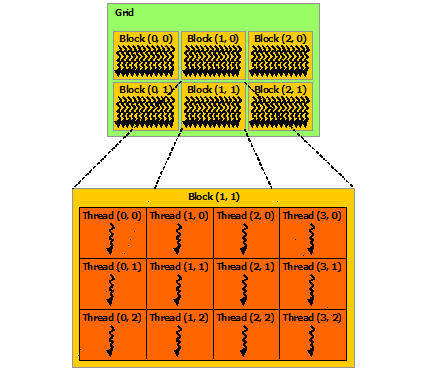
\includegraphics[width=.7\textwidth]{grid-of-thread-blocks}

    \tiny{Fonte: \url{docs.nvidia.com/cuda/cuda-c-programming-guide/index.html\#programming-model} [Acessado em 29/07/16]}
\end{frame}

\begin{frame}
    \frametitle{Relembrando: SM da arquitetura Pascal GP100}
    \centering
    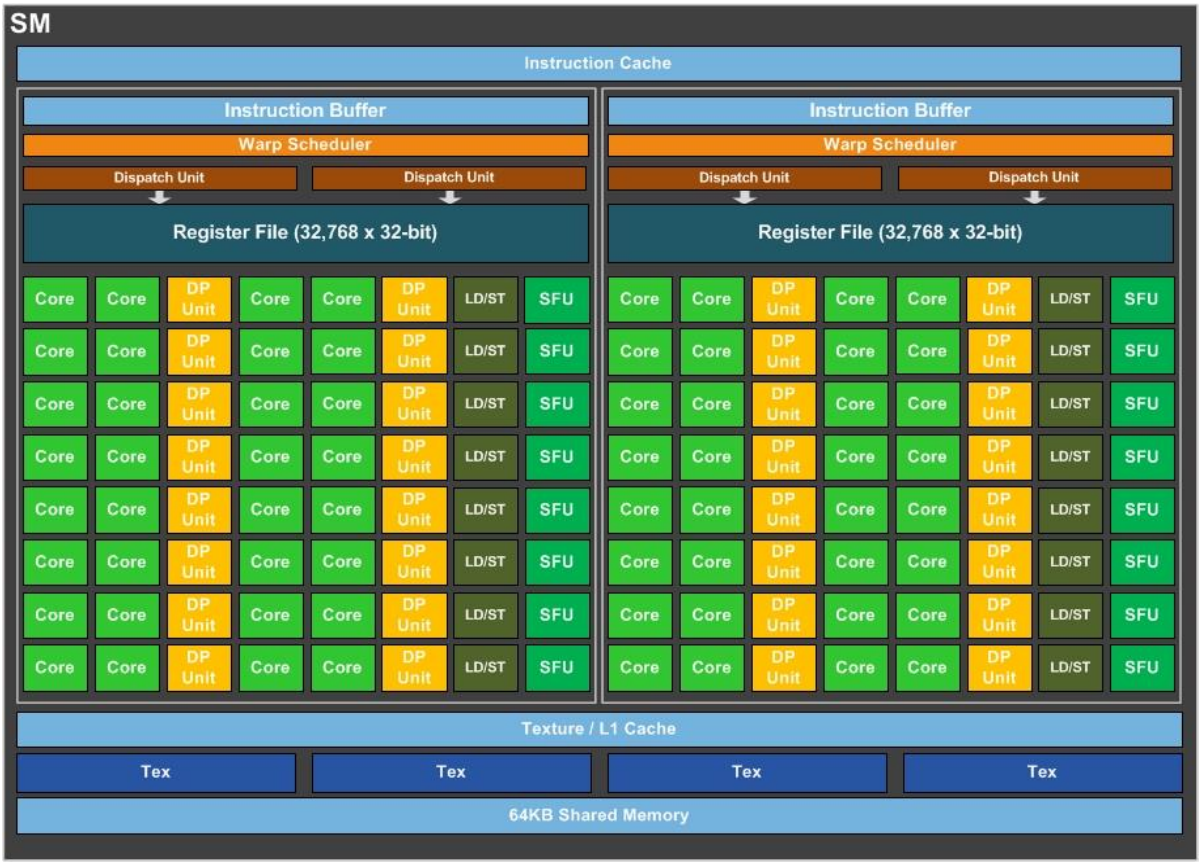
\includegraphics[width=.9\textwidth]{gp100_SM_diagram}

    \vfill

    \tiny{Imagem: \url{images.nvidia.com/content/pdf/tesla/whitepaper/pascal-architecture-whitepaper.pdf} [Acessado em 29/07/16]}
\end{frame}

\begin{frame}[fragile]
    \frametitle{CUDA C: Hierarquia de \textit{Threads}}
    \begin{lstlisting}
    __global__ void MatAdd(float A[N][N], float B[N][N], float C[N][N]) {
        int i = threadIdx.x;
        int j = threadIdx.y;
        C[i][j] = A[i][j] + B[i][j];
    }
    \end{lstlisting}
    \pause
    \begin{lstlisting}
    int main() {
        ...
        int numBlocks = 1;
        dim3 threadsPerBlock(N, N);
        MatAdd<<<numBlocks, threadsPerBlock>>>(A, B, C);
        ...
    }
    \end{lstlisting}
    \vfill

    \begin{center}
        \tiny{Fonte: \url{docs.nvidia.com/cuda/cuda-c-programming-guide/index.html\#programming-model} [Acessado em 29/07/16]}
    \end{center}
\end{frame}

\begin{frame}[fragile]
    \frametitle{CUDA C: Hierarquia de \textit{Threads}}
    \begin{lstlisting}
    __global__ void MatAdd(float A[N][N], float B[N][N], float C[N][N]) {
        int i = blockIdx.x * blockDim.x + threadIdx.x;
        int j = blockIdx.y * blockDim.y + threadIdx.y;
        if (i < N && j < N) {
            C[i][j] = A[i][j] + B[i][j];
        }
    }
    \end{lstlisting}
    \pause
    \begin{lstlisting}
    int main() {
        ...
        dim3 threadsPerBlock(16, 16);
        dim3 numBlocks(N / threadsPerBlock.x, N / threadsPerBlock.y);
        MatAdd<<<numBlocks, threadsPerBlock>>>(A, B, C);
        ...
    }
    \end{lstlisting}
    \vfill

    \begin{center}
        \tiny{Fonte: \url{docs.nvidia.com/cuda/cuda-c-programming-guide/index.html\#programming-model} [Acessado em 29/07/16]}
    \end{center}
\end{frame}

\begin{frame}[fragile]
    \frametitle{CUDA C: Hierarquia de \textit{Threads}}
    Sobre a sintaxe de lançamento e configuração \texttt{\scriptsize{\alert{<<<} Dg, Db, Ns, S \alert{>>>}}}:
    \begin{itemize}
        \item \texttt{\alert{dim3} Dg} determina dimensão e tamanho do \textit{grid}:
\begin{lstlisting}
Dg.x * Dg.y * Dg.z = numBlocks
\end{lstlisting}
        \pause
        \item \texttt{\alert{dim3} Db} determina dimensão e tamanho de cada \textit{block}:
\begin{lstlisting}
Db.x * Db.y * Db.z = threadsPerBlock
\end{lstlisting}
        \pause
        \item \texttt{\alert{size\_t} Ns = 0}: \textit{Bytes} extras na memória compartilhada
        \item \texttt{\alert{cudaStream\_t} S = 0}: CUDA \textit{stream}
    \end{itemize}

    \vfill

    \begin{center}
        \tiny{Fonte: \url{docs.nvidia.com/cuda/cuda-c-programming-guide/index.html\#programming-model} [Acessado em 29/07/16]}
    \end{center}
\end{frame}

\subsection{Hierarquia de Memória}

\begin{frame}
    \frametitle{CUDA C: Hierarquia de Memória}
    \textit{Threads} acessam \alert{múltiplos espaços de memória} durante a execução de
    um \textit{kernel}:
    \begin{itemize}
        \item Local
            \pause
        \item Compartilhada com o \textit{block}
            \pause
        \item Global\pause: persistente entre \textit{kernels} da \alert{mesma aplicação}
            \pause
        \item \textit{Read-only}
    \end{itemize}
    \vfill

    \begin{center}
        \tiny{Fonte: \url{docs.nvidia.com/cuda/cuda-c-programming-guide/index.html\#programming-model} [Acessado em 29/07/16]}
    \end{center}
\end{frame}

\begin{frame}
    \frametitle{CUDA C: Hierarquia de Memória}
    \begin{center}
        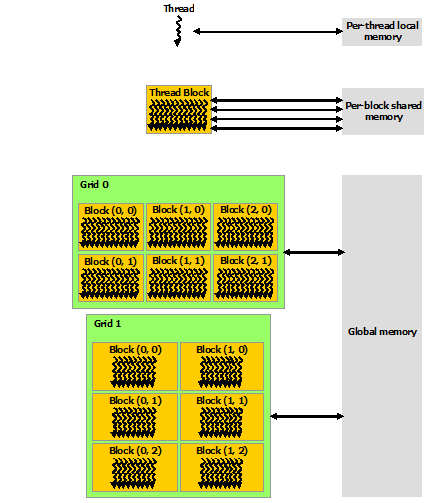
\includegraphics[width=.5\textwidth]{cuda-memory-hierarchy}
    \end{center}

    \vfill

    \begin{center}
        \tiny{Fonte: \url{docs.nvidia.com/cuda/cuda-c-programming-guide/index.html\#programming-model} [Acessado em 29/07/16]}
    \end{center}
\end{frame}

\subsection{Programação Heterogênea}

\begin{frame}
    \frametitle{CUDA C: Programação Heterogênea}
    Tarefas do \alert{host}:
    \begin{itemize}
        \item Alocar memória e recursos do \alert{device}
        \item Mover \alert{dados} (\alert{gargalo!})
            \pause
        \item Lançar \textit{kernel}
            \pause
        \item Mover \alert{resultados} (\alert{gargalo!})
        \item Liberar memória do \alert{device}
    \end{itemize}
    \pause
    Tarefas do \alert{device}:
    \begin{itemize}
        \item Executar \textit{kernel}
    \end{itemize}
\end{frame}

\begin{frame}
    \frametitle{CUDA C: Programação Heterogênea}
    \centering
    
\includegraphics[width=.8\textwidth]{accel}
\end{frame}

\subsection{Exemplo: Adição de Vetores}

\begin{frame}[fragile]
    \frametitle{Exemplo: Adição de Vetores}
    \begin{lstlisting}
    __global__ void vectorAdd(const float *A, const float *B, float *C, int numElements) {
        int i = blockDim.x * blockIdx.x + threadIdx.x;

        if (i < numElements) {
            C[i] = A[i] + B[i];
        }
    }
    \end{lstlisting}

    \vfill

    \begin{center}
        \tiny{Fonte: \url{github.com/phrb/intro-cuda} [Acessado em 29/07/16]}
    \end{center}
\end{frame}

\begin{frame}[fragile]
    \frametitle{Exemplo: Adição de Vetores}
    \begin{lstlisting}[basicstyle=\ttfamily\scriptsize]
    #include <cuda_runtime.h>
    \end{lstlisting}
    \pause
    \begin{lstlisting}[basicstyle=\ttfamily\scriptsize]
    float *h_A = (float *) malloc(size);
    if (h_A == NULL) { ... };

    float *d_A = NULL;
    err = cudaMalloc((void **) &d_A, size);
    err = cudaMemcpy(d_A, h_A, size, cudaMemcpyHostToDevice);
    if (err != cudaSuccess) { ... };
    \end{lstlisting}
    \pause
    \begin{lstlisting}[basicstyle=\ttfamily\scriptsize]
    int threadsPerBlock = 256;
    int blocksPerGrid = (numElements + threadsPerBlock - 1) / threadsPerBlock;
    \end{lstlisting}
    \pause
    \begin{lstlisting}[basicstyle=\ttfamily\scriptsize]
    vectorAdd<<<blocksPerGrid, threadsPerBlock>>>(d_A, d_B, d_C, numElements);

    err = cudaGetLastError()
    err = cudaDeviceSynchronize()
    if (err != cudaSuccess) { ... };
    \end{lstlisting}
    \pause
    \begin{lstlisting}[basicstyle=\ttfamily\scriptsize]
    err = cudaMemcpy(h_C, d_C, size, cudaMemcpyDeviceToHost);
    err = cudaFree(d_A);
    if (err != cudaSuccess) { ... };
    \end{lstlisting}

    \vfill

    \begin{center}
        \tiny{Fonte: \url{github.com/phrb/intro-cuda} [Acessado em 29/07/16]}
    \end{center}
\end{frame}

\begin{frame}[fragile]
    \frametitle{Exemplo: Dica Prática}
    \alert{Sempre} procure por erros!

    \begin{lstlisting}
    float *d_A = NULL;
    err = cudaMalloc((void **) &d_A, size);

    err = cudaGetLastError()

    err = cudaDeviceSynchronize()
    \end{lstlisting}
    \pause
    \begin{lstlisting}
    if (err != cudaSuccess) {
        fprintf(stderr, "Failed to allocate device vector A (error code %s)!\n", cudaGetErrorString(err));
        exit(EXIT_FAILURE);
    }
    \end{lstlisting}

    \begin{center}
        \tiny{Fonte: \url{github.com/phrb/intro-cuda} [Acessado em 29/07/16]}
    \end{center}
\end{frame}

\subsection{Mão na massa!}

\begin{frame}
    \frametitle{Mão na massa!}
    Vamos executar alguns exemplos em CUDA C,
    disponíveis em \url{github.com/phrb/intro-cuda}:
    \begin{itemize}
        \item \url{src/cuda-samples/0_Simple/vectorAdd}
            \pause
        \item \url{src/cuda-samples/5_Simulations/fluidsGL}
        \item \url{src/cuda-samples/5_Simulations/oceanFFT}
        \item \url{src/cuda-samples/5_Simulations/smokeParticles}
            \pause
        \item \url{src/mandelbrot_numba}
    \end{itemize}
\end{frame}

\subsection{Recursos}

\begin{frame}
    \frametitle{Recursos}
    O \emph{pdf} com as aulas e todo o código fonte estão no \alert{GitHub}:

    \begin{itemize}
        \item \url{github.com/phrb/intro-cuda}
    \end{itemize}

    Outros recursos:

    \begin{itemize}
        \item CUDA C: \url{docs.nvidia.com/cuda/cuda-c-programming-guide}
        \item CUDA Toolkit: \url{developer.nvidia.com/cuda-toolkit}
        \item Guia de Boas Práticas:
            \begin{itemize}
                \item \url{docs.nvidia.com/cuda/cuda-c-best-practices-guide}
            \end{itemize}
        \item GPU Teaching Kit: \url{syllabus.gputeachingkit.com}
        \item iPython: \url{ipython.org/notebook.html}
        \item Anaconda: \url{continuum.io/downloads}
    \end{itemize}
\end{frame}

\part{Parte II}

\maketitle

\section{Retomada}

\subsection{Sobre}

\begin{frame}
    \frametitle{Sobre}
    \begin{columns}[T,onlytextwidth]
        \column{0.5\textwidth}
        \begin{center}
            
\includegraphics[width=.45\textwidth]{pedro}

            Pedro Bruel
        \end{center}

        \begin{itemize}
            \item \alert{phrb}@ime.usp.br
            \item \url{www.ime.usp.br/~phrb}
            \item \url{github.com/phrb}
        \end{itemize}

        \column{0.5\textwidth}
        \begin{center}
            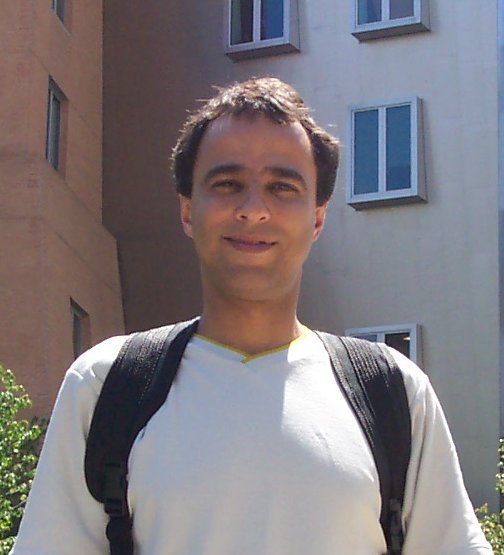
\includegraphics[width=.4\textwidth]{alfredo}

            Alfredo Goldman
        \end{center}

        \begin{itemize}
            \item \alert{gold}@ime.usp.br
            \item \url{www.ime.usp.br/~gold}
        \end{itemize}
    \end{columns}
\end{frame}

\begin{frame}
    \frametitle{Pesquisa}
    Meus interesses de \alert{pesquisa}:
    \begin{itemize}
        \item \textit{Autotuning}
        \item \textit{Stochastic Local Search}
        \item \textit{Model Based Search}
        \item GPUs, FPGAs, \textit{cloud}
        \item Julia Language
        \item Colaboração! (\alert{phrb@ime.usp.br})
    \end{itemize}
\end{frame}

\subsection{Roteiro}

\begin{frame}
    \frametitle{Parte I}
    \setbeamertemplate{section in toc}[sections numbered]
    \tableofcontents[hideallsubsections, part=1]
\end{frame}

\begin{frame}
    \frametitle{Parte II}
    \setbeamertemplate{section in toc}[sections numbered]
    \tableofcontents[hideallsubsections, part=2]
\end{frame}

\begin{frame}
    \frametitle{Slides}
    \begin{center}
        
\includegraphics[width=.18\textwidth]{github}
    \end{center}
    O \emph{pdf} com as aulas e todo o código fonte estão no \alert{GitHub}:

    \begin{itemize}
        \item \url{github.com/phrb/intro-cuda}
    \end{itemize}
\end{frame}

\subsection{Relembrando}

\begin{frame}
    \frametitle{Aceleração por \textit{Hardware}}
    \begin{center}
        
\includegraphics[width=.6\textwidth]{accelerate}
    \end{center}

    Uso de \alert{dispositivos} (devices) para acelerar computações aplicadas a
    grandes conjuntos de dados:

    \begin{itemize}
        \item Associação a um processador \alert{hospedeiro} (host)
        \item Controle e memória próprios
        \item Diferem em especialização e configurabilidade
        \item \alert{GPUs}, DSPs, FPGAs, ASICs
    \end{itemize}
\end{frame}

\begin{frame}
    \frametitle{Aceleração por \textit{Hardware}}
    \centering
    
\includegraphics[width=.8\textwidth]{accel}
\end{frame}

\begin{frame}
    \frametitle{Aceleração por \textit{Hardware}}
    Porcentagem de sistemas com aceleradores na \textit{Top500}:

    \begin{center}
    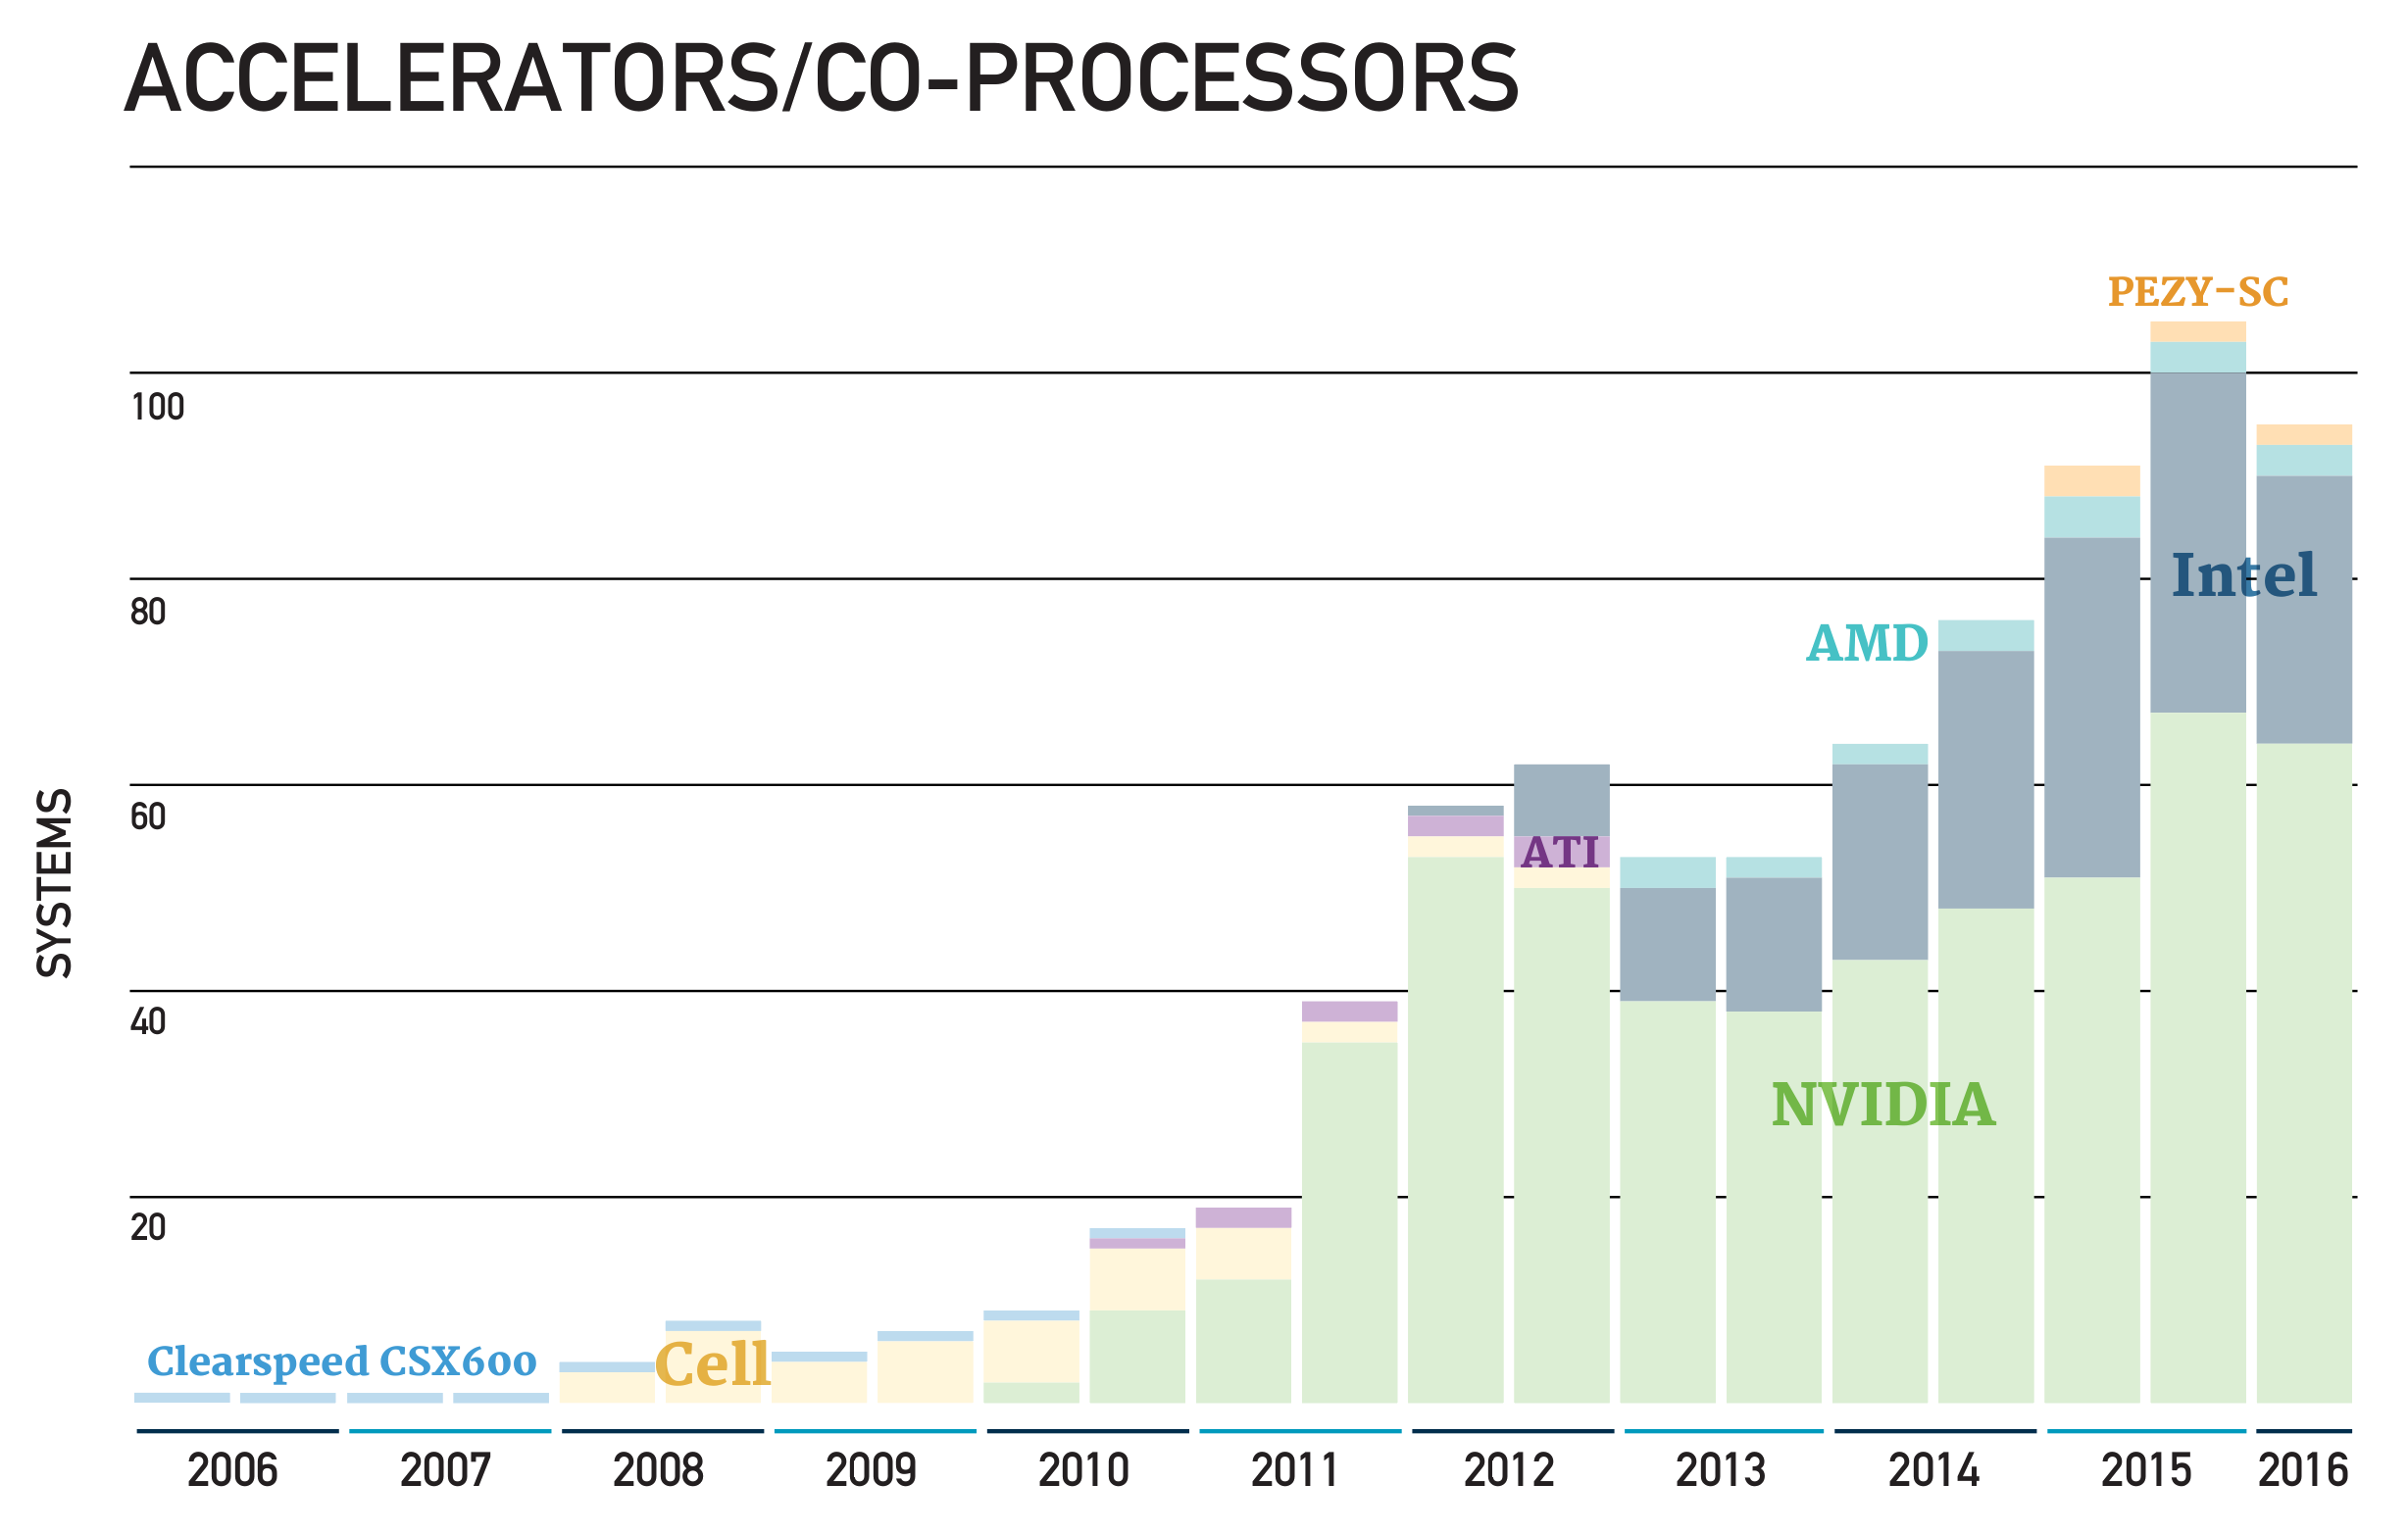
\includegraphics[width=.95\textwidth]{top500_accel}
    \hfill

        \tiny{Imagem: \url{top500.org/lists/2016/06/download/TOP500_201606_Poster.pdf} [Acessado em 29/07/16]}
    \end{center}
\end{frame}

\begin{frame}
    \frametitle{Computação Heterogênea}
    \begin{center}
        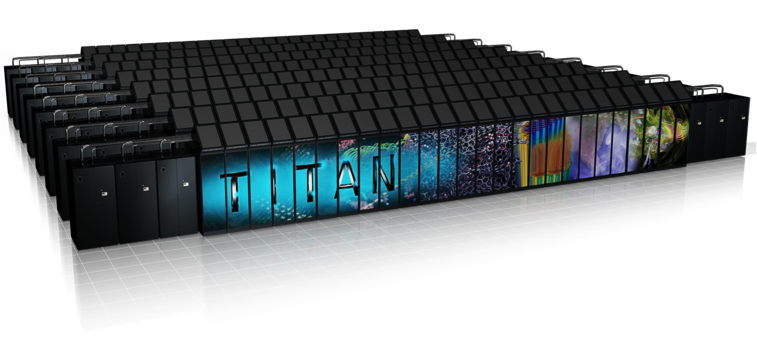
\includegraphics[width=.7\textwidth]{titan}
    \end{center}

    Dados recursos computacionais \alert{heterogêneos}, conjuntos de
    \alert{dados} e \alert{computações}, como distribuir computações e dados de
    forma a \alert{otimizar o uso} dos recursos?
    \hfill

    \begin{center}
    \tiny{Imagem: \url{olcf.ornl.gov/titan} [Acessado em 29/07/16]}
    \end{center}
\end{frame}

\begin{frame}
    \frametitle{Graphics Processing Units}
    \begin{center}
        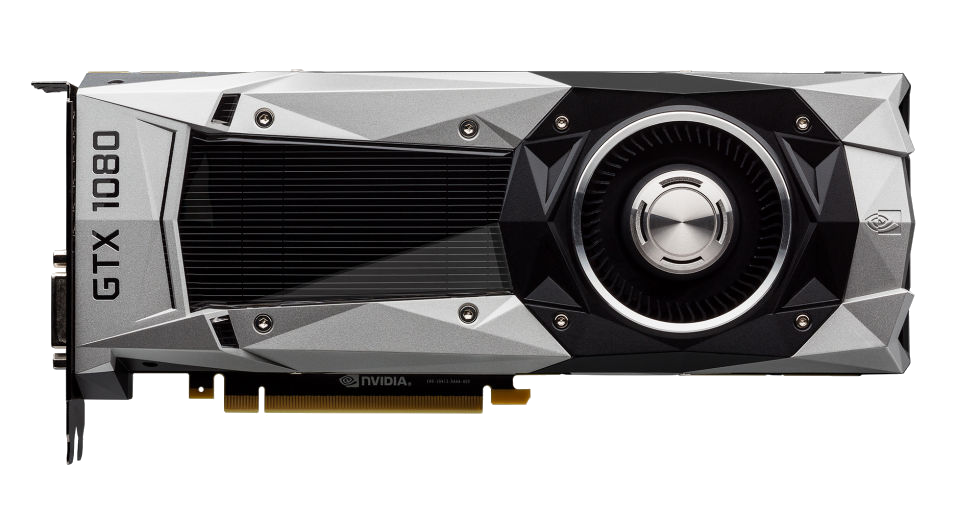
\includegraphics[width=.6\textwidth]{gtx1080}
    \end{center}

    Originalmente especializadas em \alert{processamento gráfico},
    trabalham com muitos dados e têm \alert{alta vazão}:
    \begin{itemize}
        \item Caches pequenos (\textit{kilobytes})
        \item Sem \alert{branch prediction}
        \item \alert{Milhares} de ALUs de \alert{maior latência}
        \item \alert{Pipelines} de execução
        \item 114 688 \alert{threads} concorrentes na arquitetura Pascal
    \end{itemize}
\end{frame}

\begin{frame}
    \frametitle{Plataforma CUDA}
    \begin{center}
        
\includegraphics[width=.4\textwidth]{cuda-logo}
    \end{center}
    \begin{itemize}
        \item Plataforma para \alert{computação paralela}
        \item \textit{Application Programming Interface} (API)
        \item CUDA \textit{Toolkit}
    \end{itemize}
\end{frame}

\begin{frame}
    \frametitle{Linguagens de Programação}
    \begin{center}
        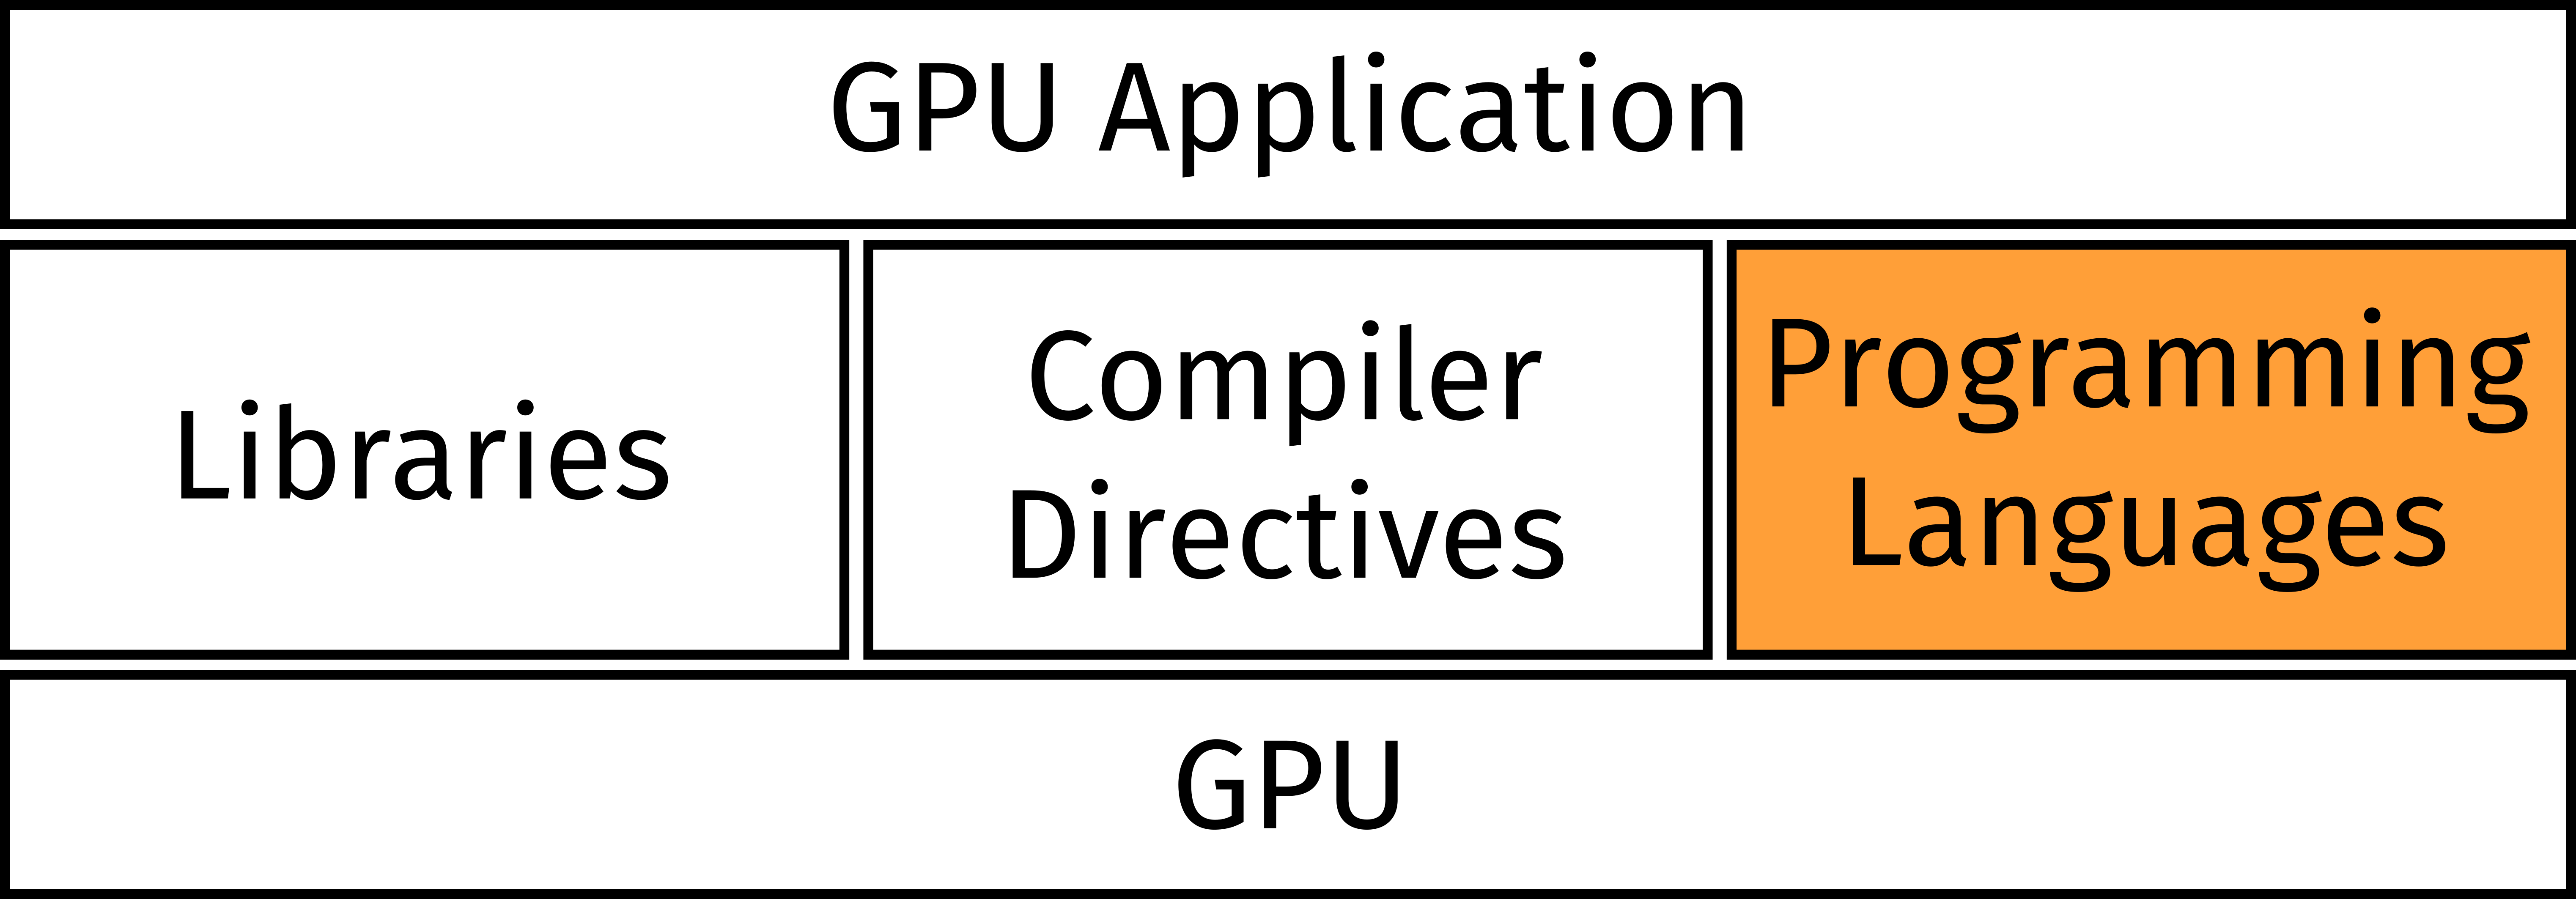
\includegraphics[width=.6\textwidth]{accel_apps_lang}
    \end{center}
    \begin{itemize}
        \item Melhor desempenho, mas mais difíceis de usar
        \item Flexíveis
    \end{itemize}
\end{frame}

\begin{frame}
    \frametitle{CUDA C}
    \begin{center}
        
\includegraphics[width=.3\textwidth]{cuda-c}
    \end{center}
    Modelo de Programação:
    \begin{itemize}
        \item \alert{Kernels}
        \item Hierarquia de \alert{Threads}
        \item Hierarquia de \alert{Memória}
        \item Programação \alert{Heterogênea}
    \end{itemize}
\end{frame}

\begin{frame}[fragile]
    \frametitle{Exemplo: Adição de Vetores}
    \begin{lstlisting}[basicstyle=\ttfamily\scriptsize]
    #include <cuda_runtime.h>

    float *h_A = (float *) malloc(size);
    if (h_A == NULL) { ... };

    float *d_A = NULL;
    err = cudaMalloc((void **) &d_A, size);
    err = cudaMemcpy(d_A, h_A, size, cudaMemcpyHostToDevice);
    if (err != cudaSuccess) { ... };

    int threadsPerBlock = 256;
    int blocksPerGrid = (numElements + threadsPerBlock - 1) / threadsPerBlock;

    vectorAdd<<<blocksPerGrid, threadsPerBlock>>>(d_A, d_B, d_C, numElements);

    err = cudaGetLastError()
    err = cudaDeviceSynchronize()
    if (err != cudaSuccess) { ... };

    err = cudaMemcpy(h_C, d_C, size, cudaMemcpyDeviceToHost);
    err = cudaFree(d_A);
    if (err != cudaSuccess) { ... };
    \end{lstlisting}

    \vfill

    \begin{center}
        \tiny{Fonte: \url{github.com/phrb/intro-cuda} [Acessado em 29/07/16]}
    \end{center}
\end{frame}

\begin{frame}
    \frametitle{Mão na massa!}
    Vamos executar alguns exemplos em CUDA C,
    disponíveis em \url{github.com/phrb/intro-cuda}:
    \begin{itemize}
        \item \url{src/cuda-samples/0_Simple/vectorAdd}
        \item \url{src/cuda-samples/5_Simulations/fluidsGL}
        \item \url{src/cuda-samples/5_Simulations/oceanFFT}
        \item \url{src/cuda-samples/5_Simulations/smokeParticles}
        \item \url{src/mandelbrot_numba}
    \end{itemize}
\end{frame}

\begin{frame}[fragile]
    \frametitle{Dica Prática}
    \alert{Sempre} procure por erros!

    \begin{lstlisting}
    float *d_A = NULL;
    err = cudaMalloc((void **) &d_A, size);

    err = cudaGetLastError()

    err = cudaDeviceSynchronize()

    if (err != cudaSuccess) {
        fprintf(stderr, "Failed to allocate device vector A (error code %s)!\n", cudaGetErrorString(err));
        exit(EXIT_FAILURE);
    }
    \end{lstlisting}

    \begin{center}
        \tiny{Fonte: \url{github.com/phrb/intro-cuda} [Acessado em 29/07/16]}
    \end{center}
\end{frame}

\section{Compilação de Aplicações CUDA}

\subsection{Nvidia CUDA Compiler}

\begin{frame}
    \frametitle{Nvidia CUDA Compiler (\texttt{nvcc})}
    \begin{center}
        
\includegraphics[width=.55\textwidth]{compiler}
    \end{center}
    \pause
    \begin{itemize}
        \item Sistema \alert{proprietário}
            \pause
        \item Usa o compilador C++ do \textit{host}
            \pause
        \item Compila código CUDA para \textit{Parallel Thread Execution} (\alert{PTX} ISA)
            \pause
        \item Código do \textit{host} + Código do \textit{device} $\rightarrow$ \alert{fatbinary}
    \end{itemize}
\end{frame}

\subsection{Modelo de Programação}

\begin{frame}
    \frametitle{\texttt{nvcc}: Modelo de programação CUDA}
    \begin{itemize}
        \item SIMD, SIMT
        \item \textit{Single Program Multiple Data} (SPMD)
            \pause
        \item \textit{Device}: \alert{threads} paralelas e \alert{independentes}
        \item \textit{Host}: não interfere
    \end{itemize}
\end{frame}

\subsection{Trajetória de Compilação}

\begin{frame}
    \frametitle{\texttt{nvcc}: Trajetória de Compilação}
    \centering
    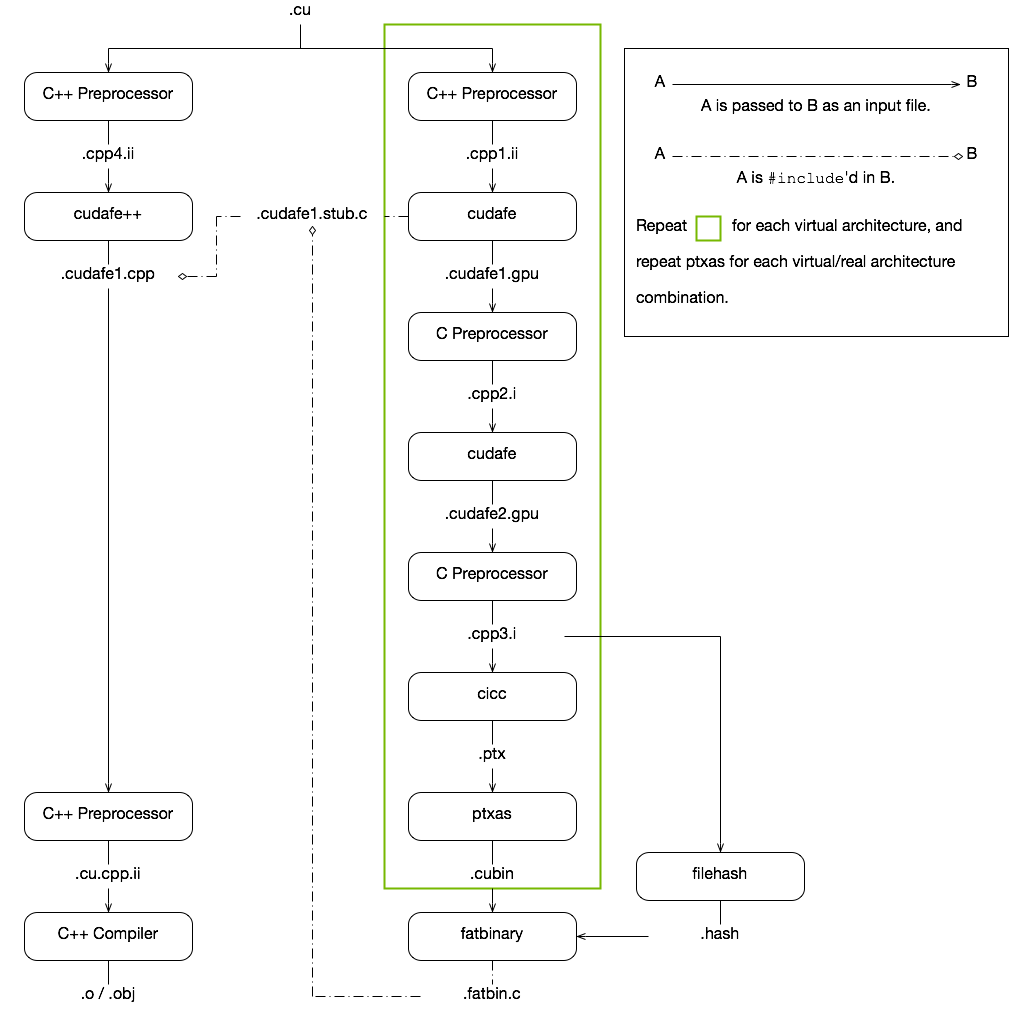
\includegraphics[width=.7\textwidth]{cuda-compilation}
    \vfill

    \begin{center}
        \tiny{Imagem: \url{docs.nvidia.com/cuda/cuda-compiler-driver-nvcc} [Acessado em 29/07/16]}
    \end{center}
\end{frame}

\section{Boas Práticas em Otimização}

\subsection{Measure, Parallelize, Optimize, Deploy}

\begin{frame}
    \frametitle{Measure, Parallelize, Optimize, Deploy}
    \centering
    
\includegraphics[width=.9\textwidth]{MPOD}
    \vfill

    \begin{center}
        \tiny{Fonte: \url{docs.nvidia.com/cuda/cuda-c-best-practices-guide} [Acessado em 29/07/16]}
    \end{center}
\end{frame}

\subsection{Measure}

\begin{frame}
    \frametitle{Measure}
    \begin{center}
    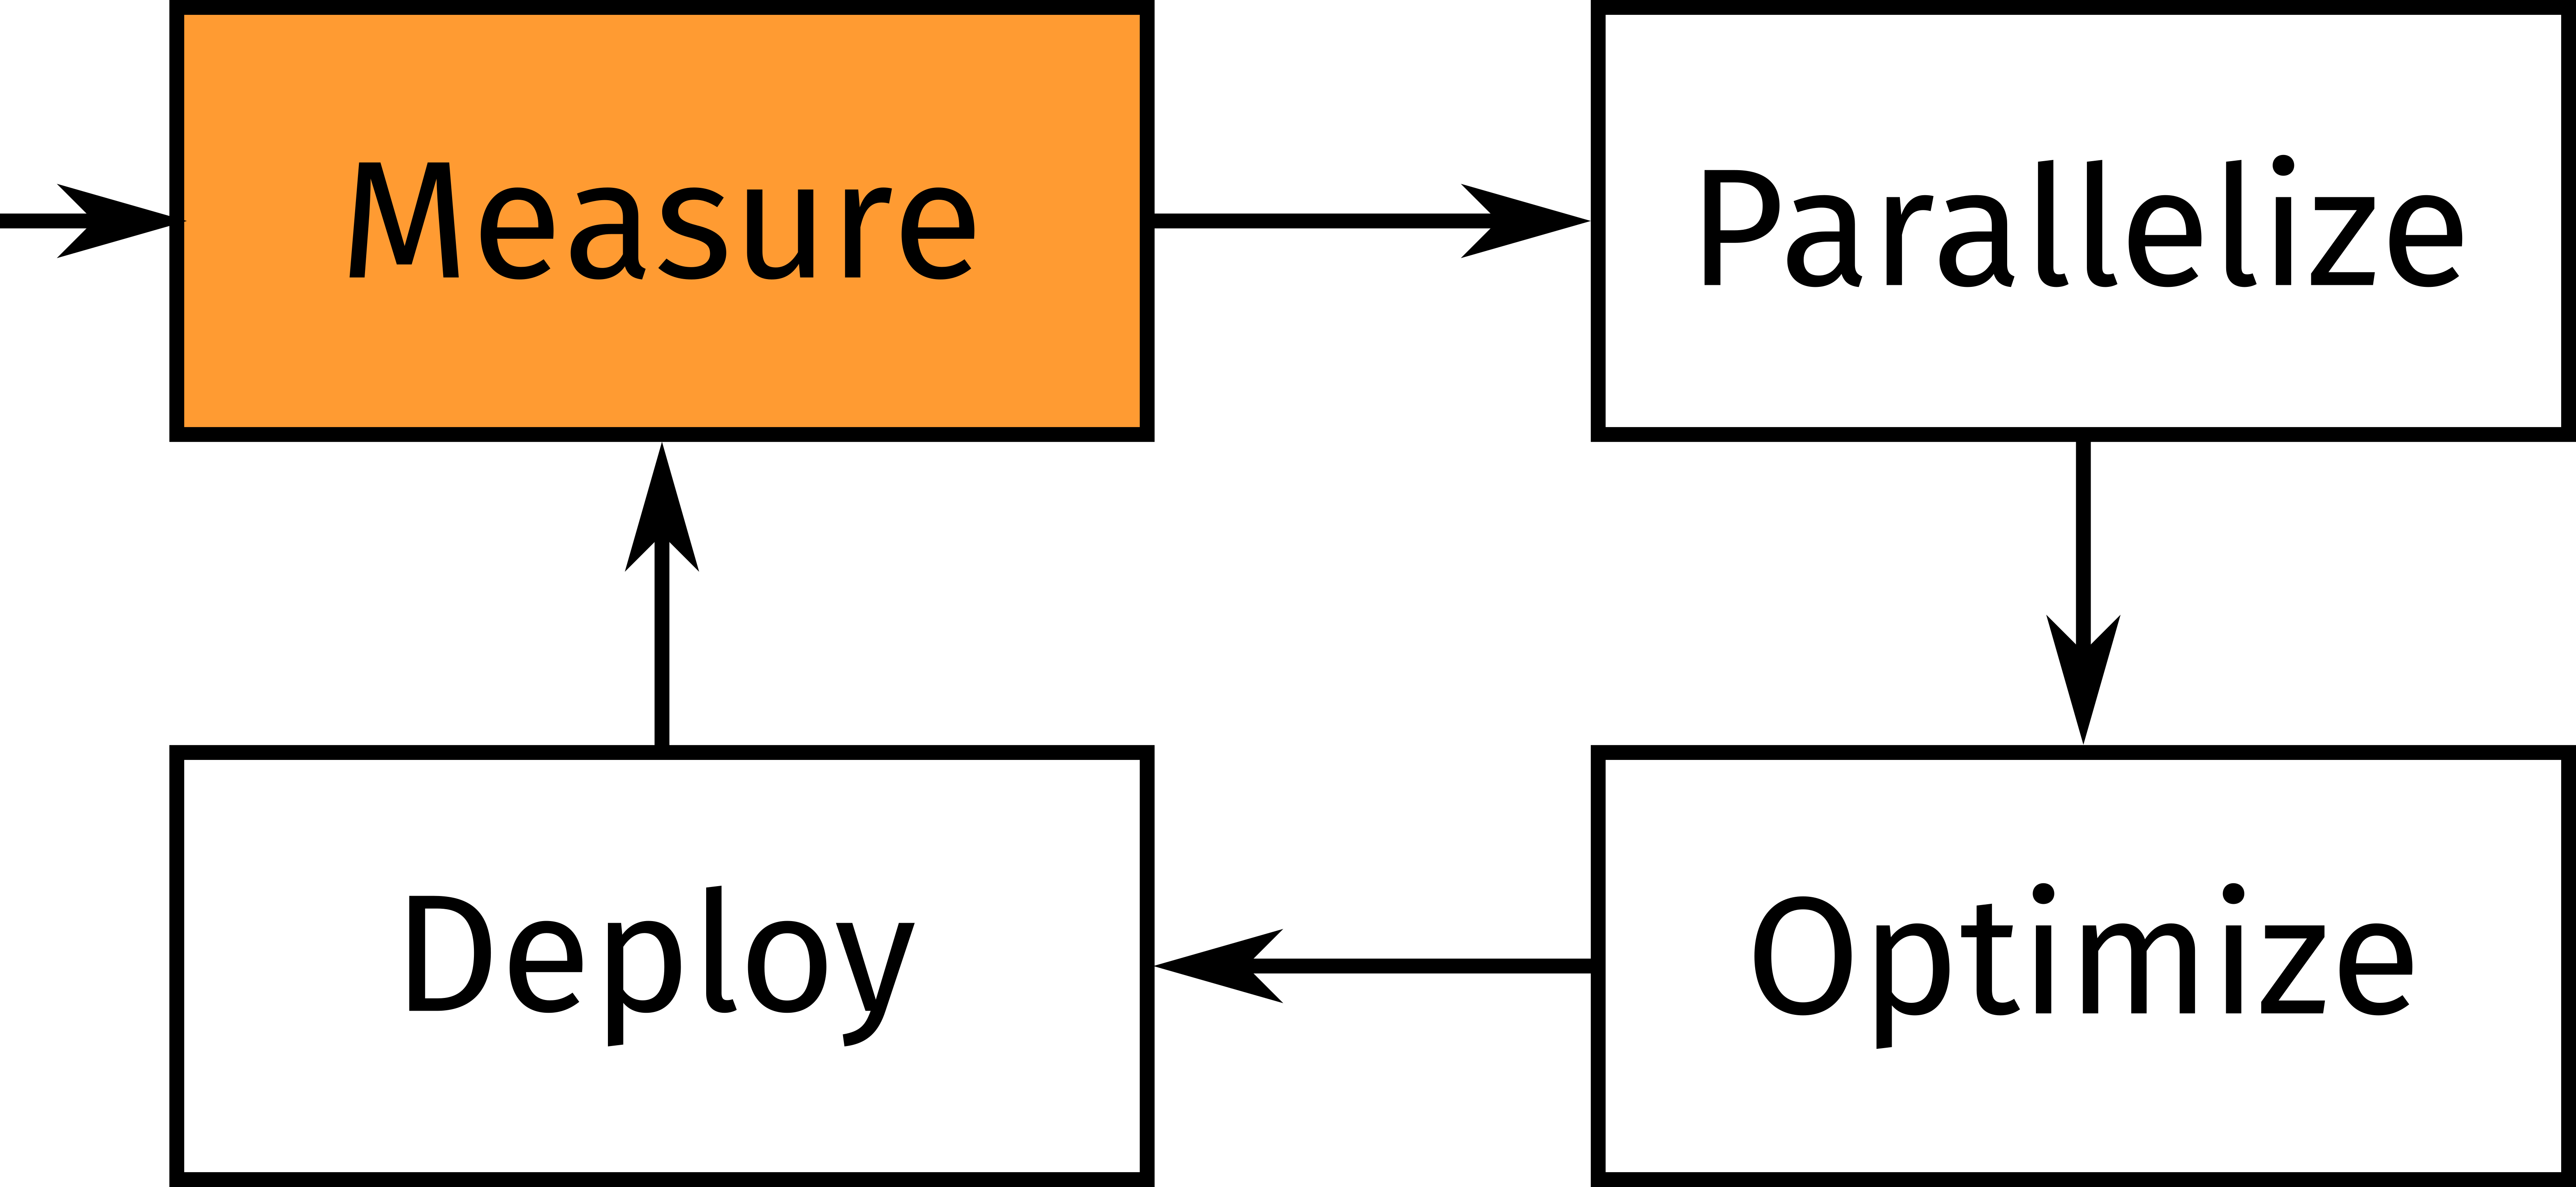
\includegraphics[width=.4\textwidth]{MPOD_M}
    \end{center}
    \vfill

    \pause
    Dado um \alert{programa sequencial}:
    \begin{itemize}
        \item Quais funções fazem o \alert{trabalho pesado} (\alert{gargalos})?
            \pause
        \item É possível \alert{paralelizá-las}?
            \pause
        \item Como o programa se comporta quando:
            \begin{itemize}
                \item O trabalho é divido entre mais processos? (\alert{strong scaling})
                    \pause
                \item Há mais trabalho a ser feito? (\alert{weak scaling})
            \end{itemize}
    \end{itemize}
\end{frame}

\subsection{Parallelize}

\begin{frame}
    \frametitle{Parallelize}
    \begin{center}
    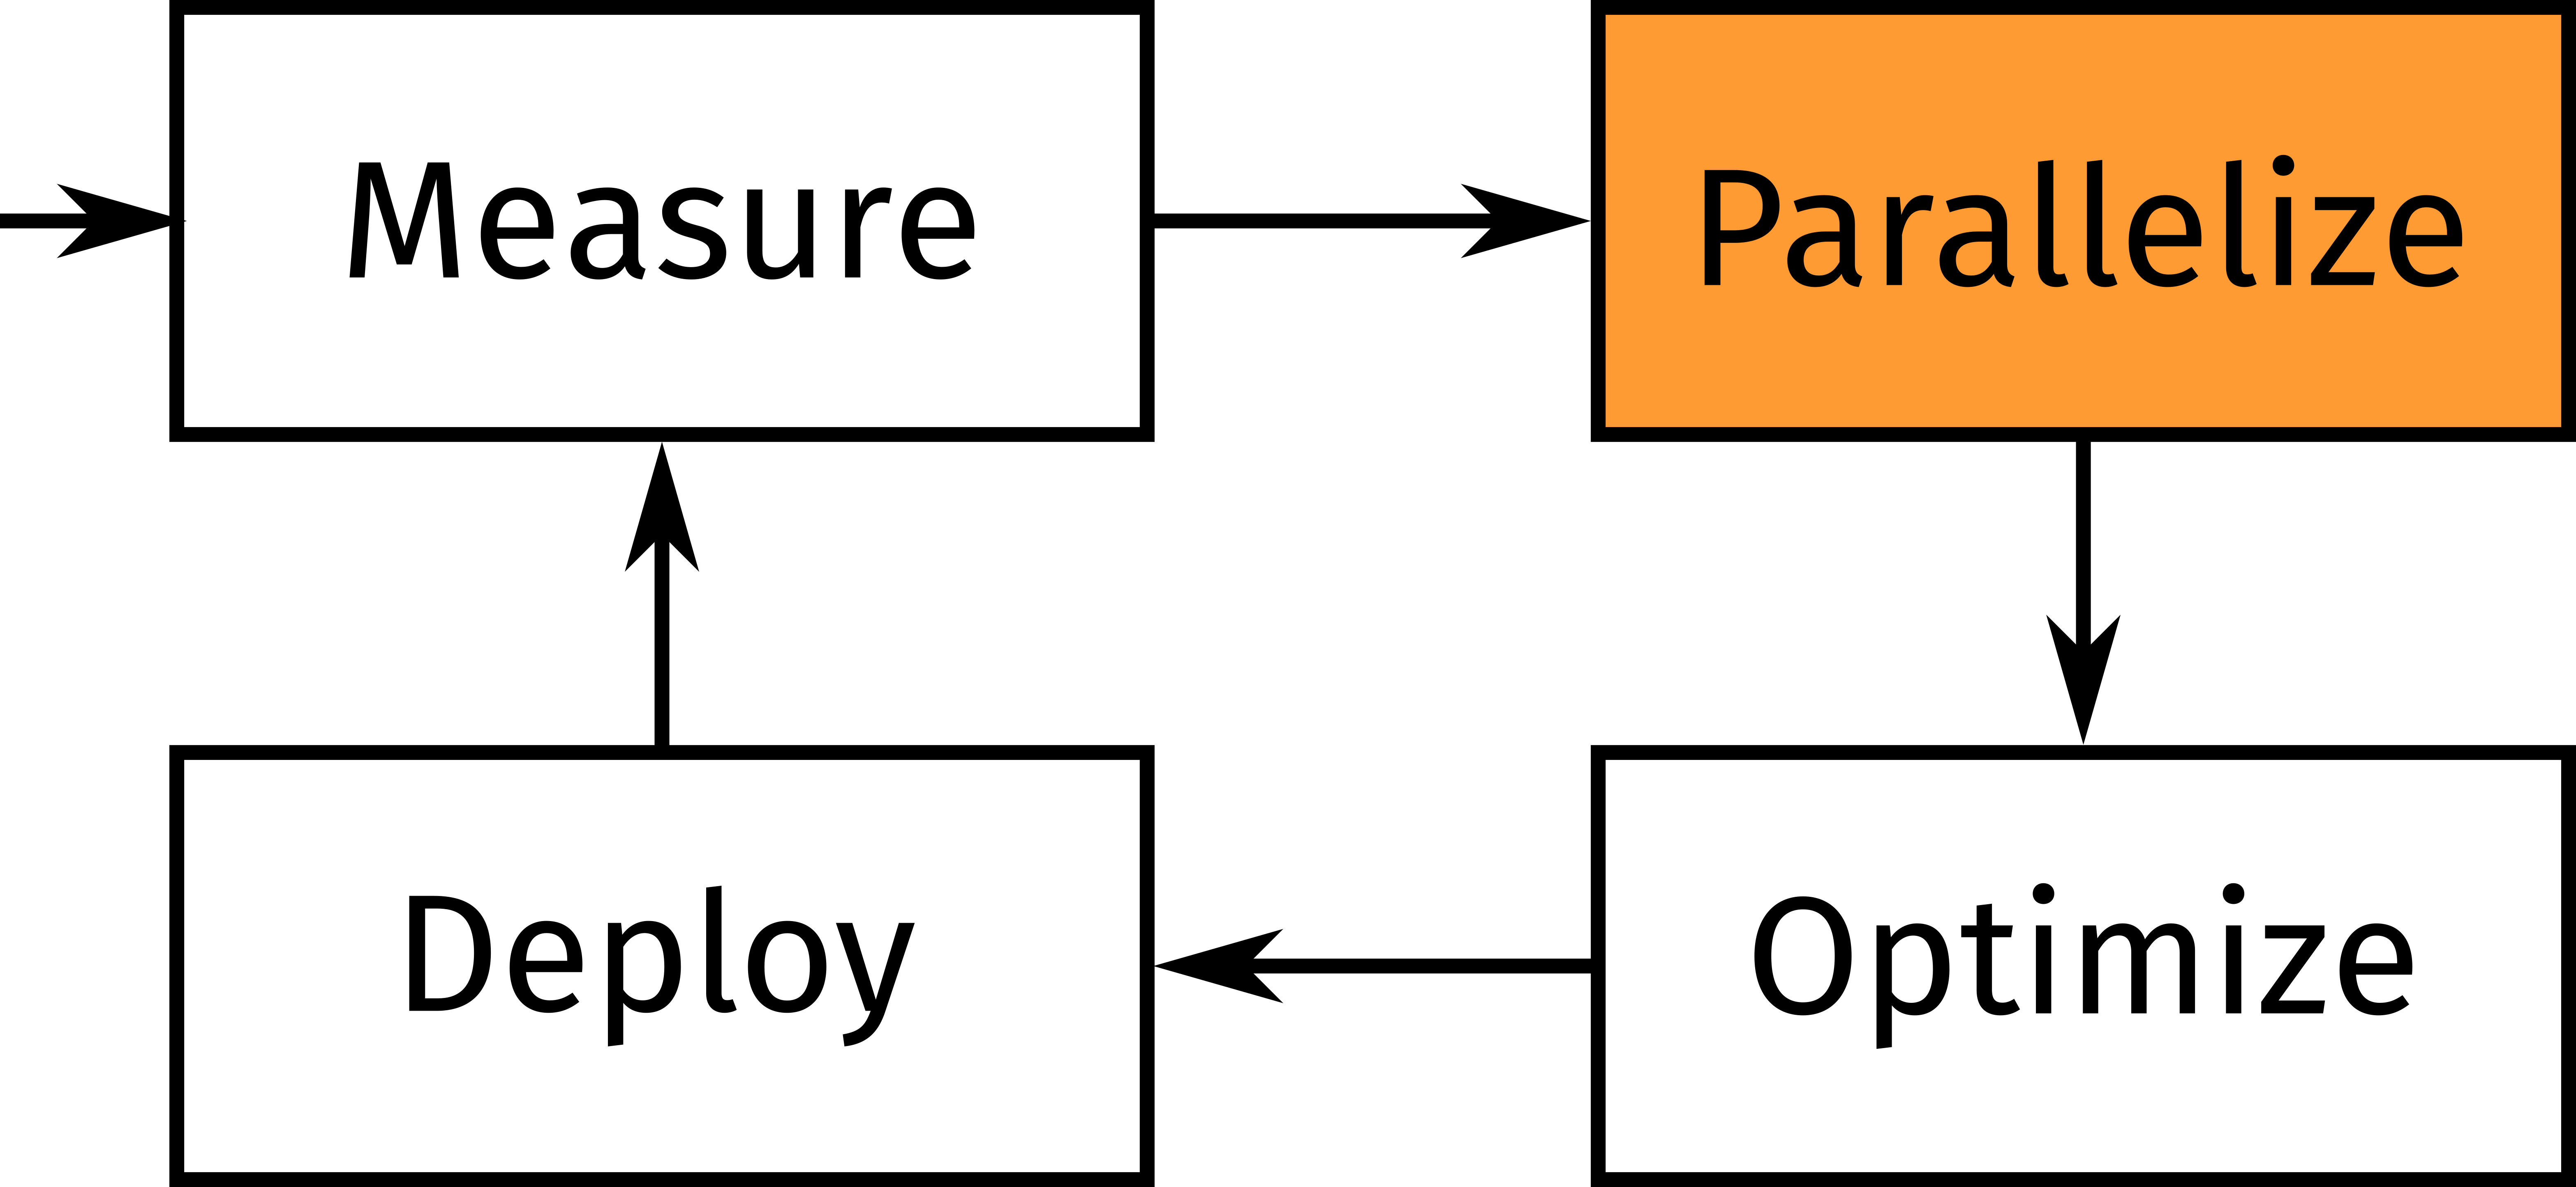
\includegraphics[width=.4\textwidth]{MPOD_P}
    \vfill
        \pause
    
\includegraphics[width=.6\textwidth]{accel_apps}
    \end{center}
\end{frame}

\begin{frame}
    \frametitle{Parallelize}
    \begin{center}
    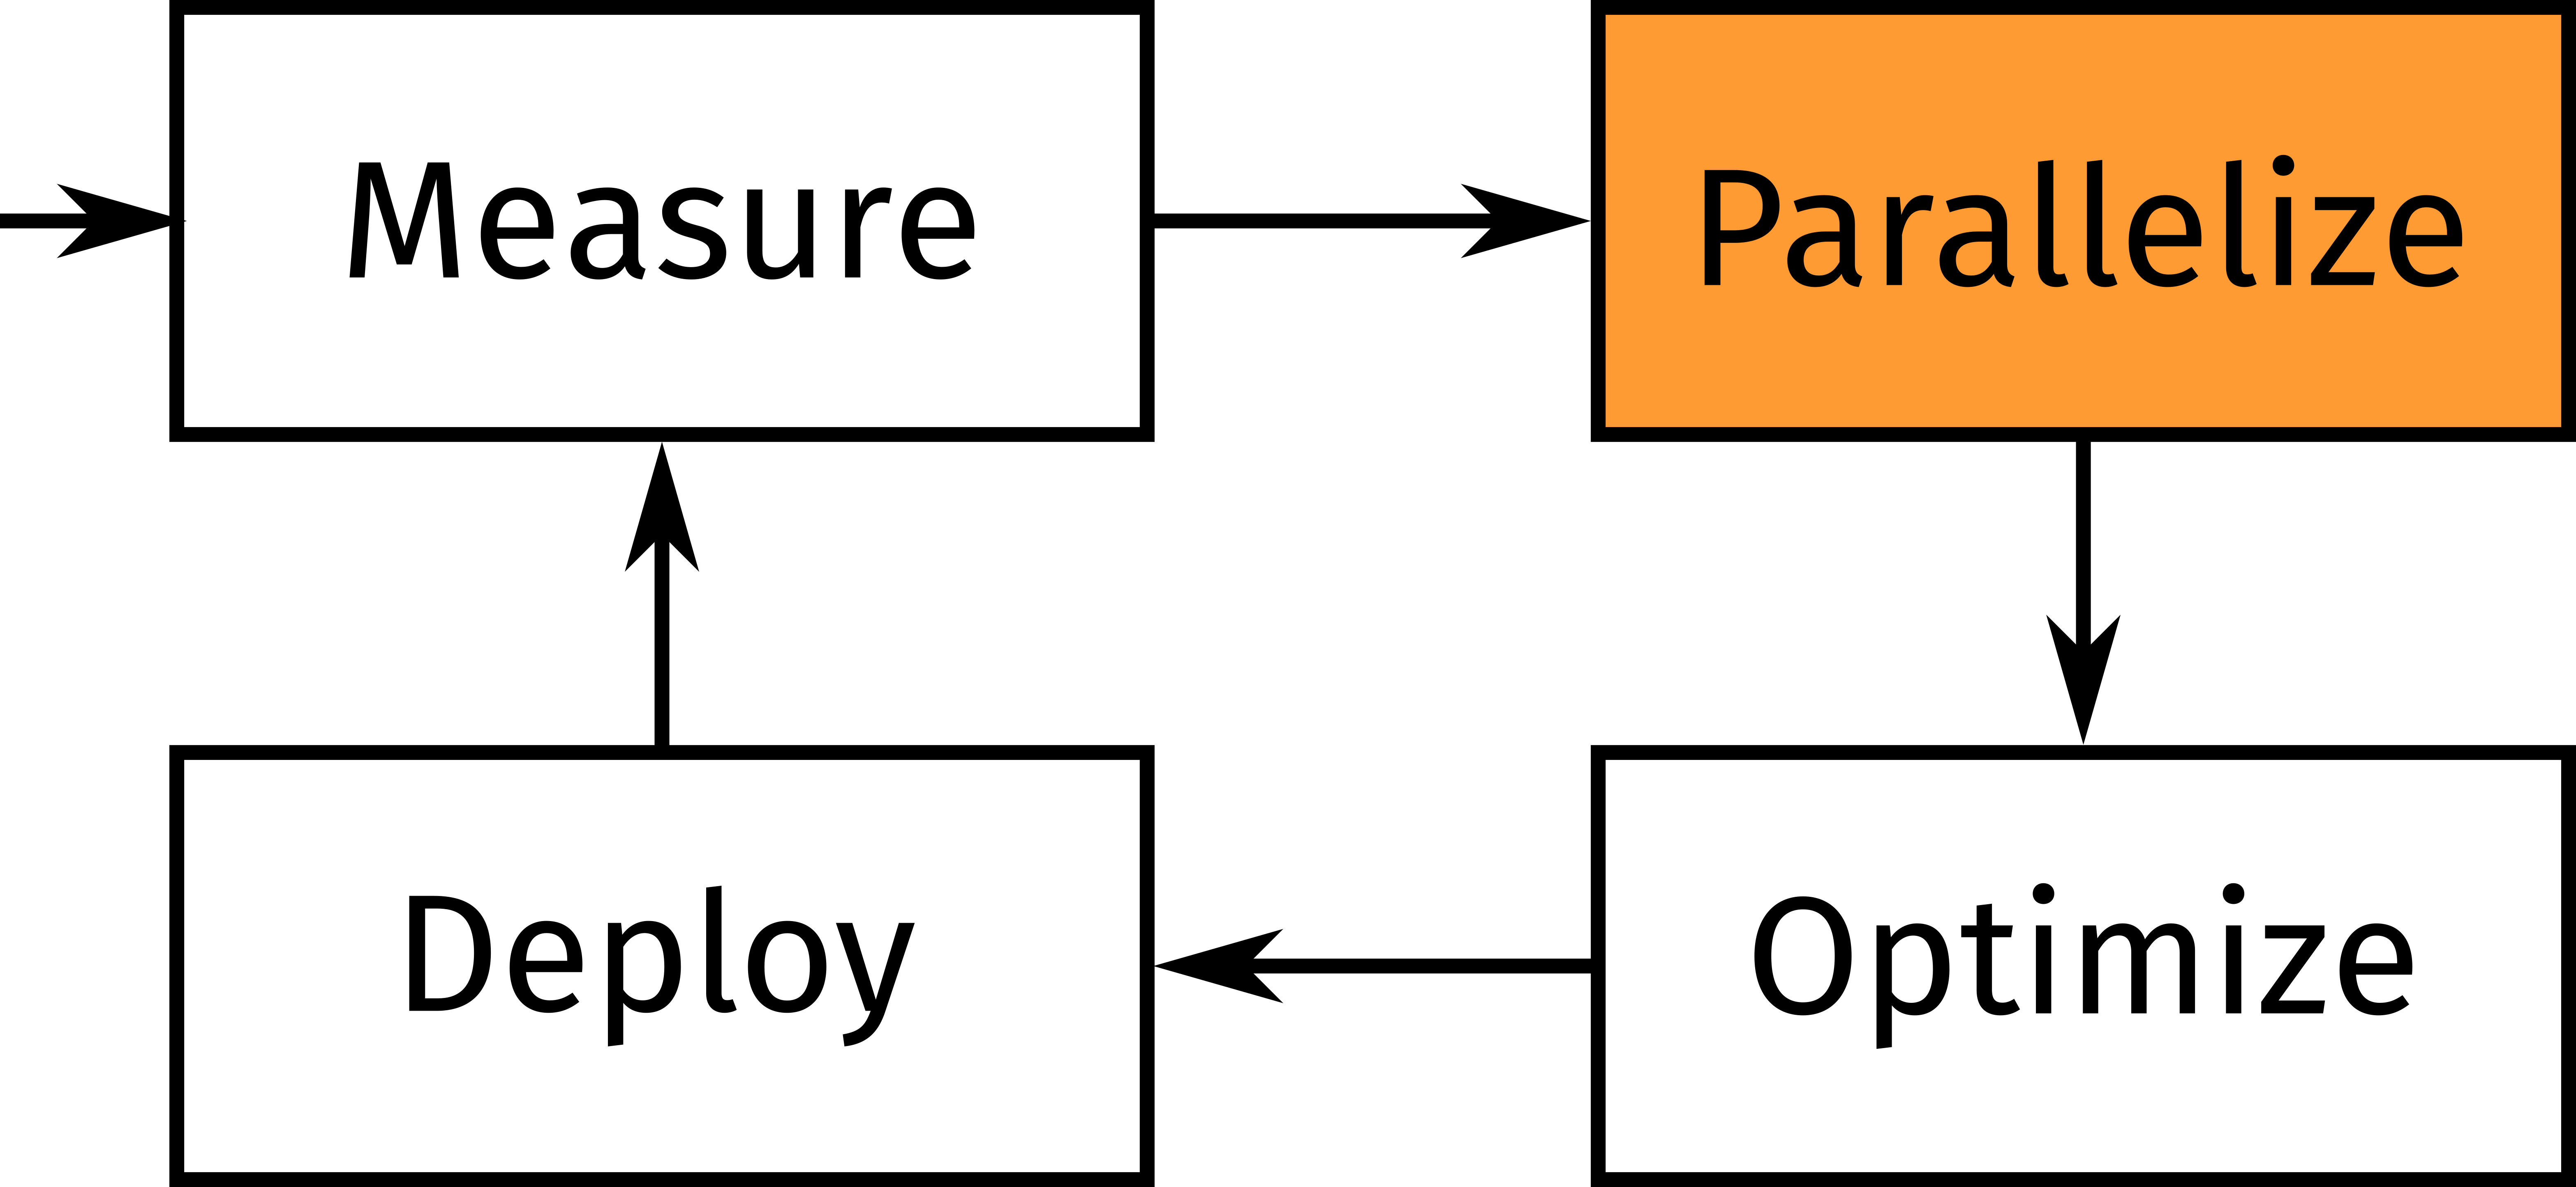
\includegraphics[width=.4\textwidth]{MPOD_P}
    \vfill
    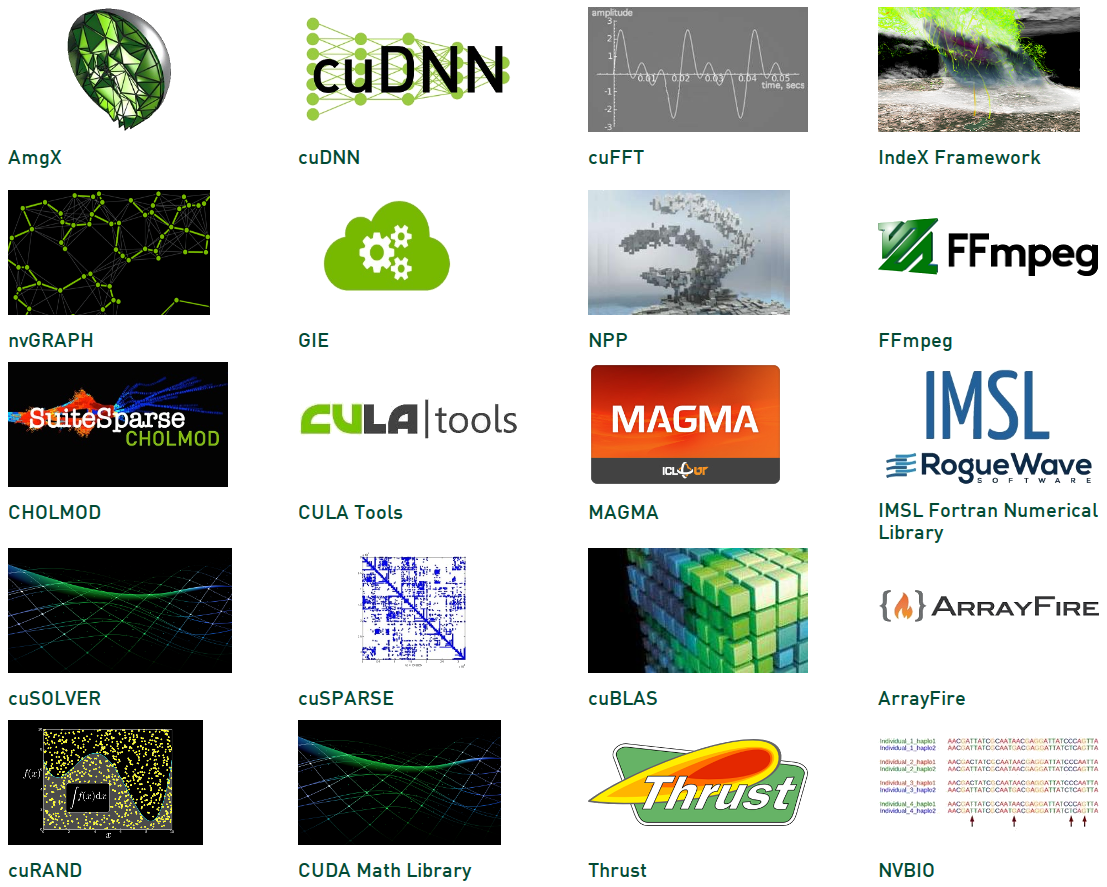
\includegraphics[width=.5\textwidth]{accel_libs_no}
    \end{center}
\end{frame}

\subsection{Optimze}

\begin{frame}
    \frametitle{Optimize}
    \begin{center}
    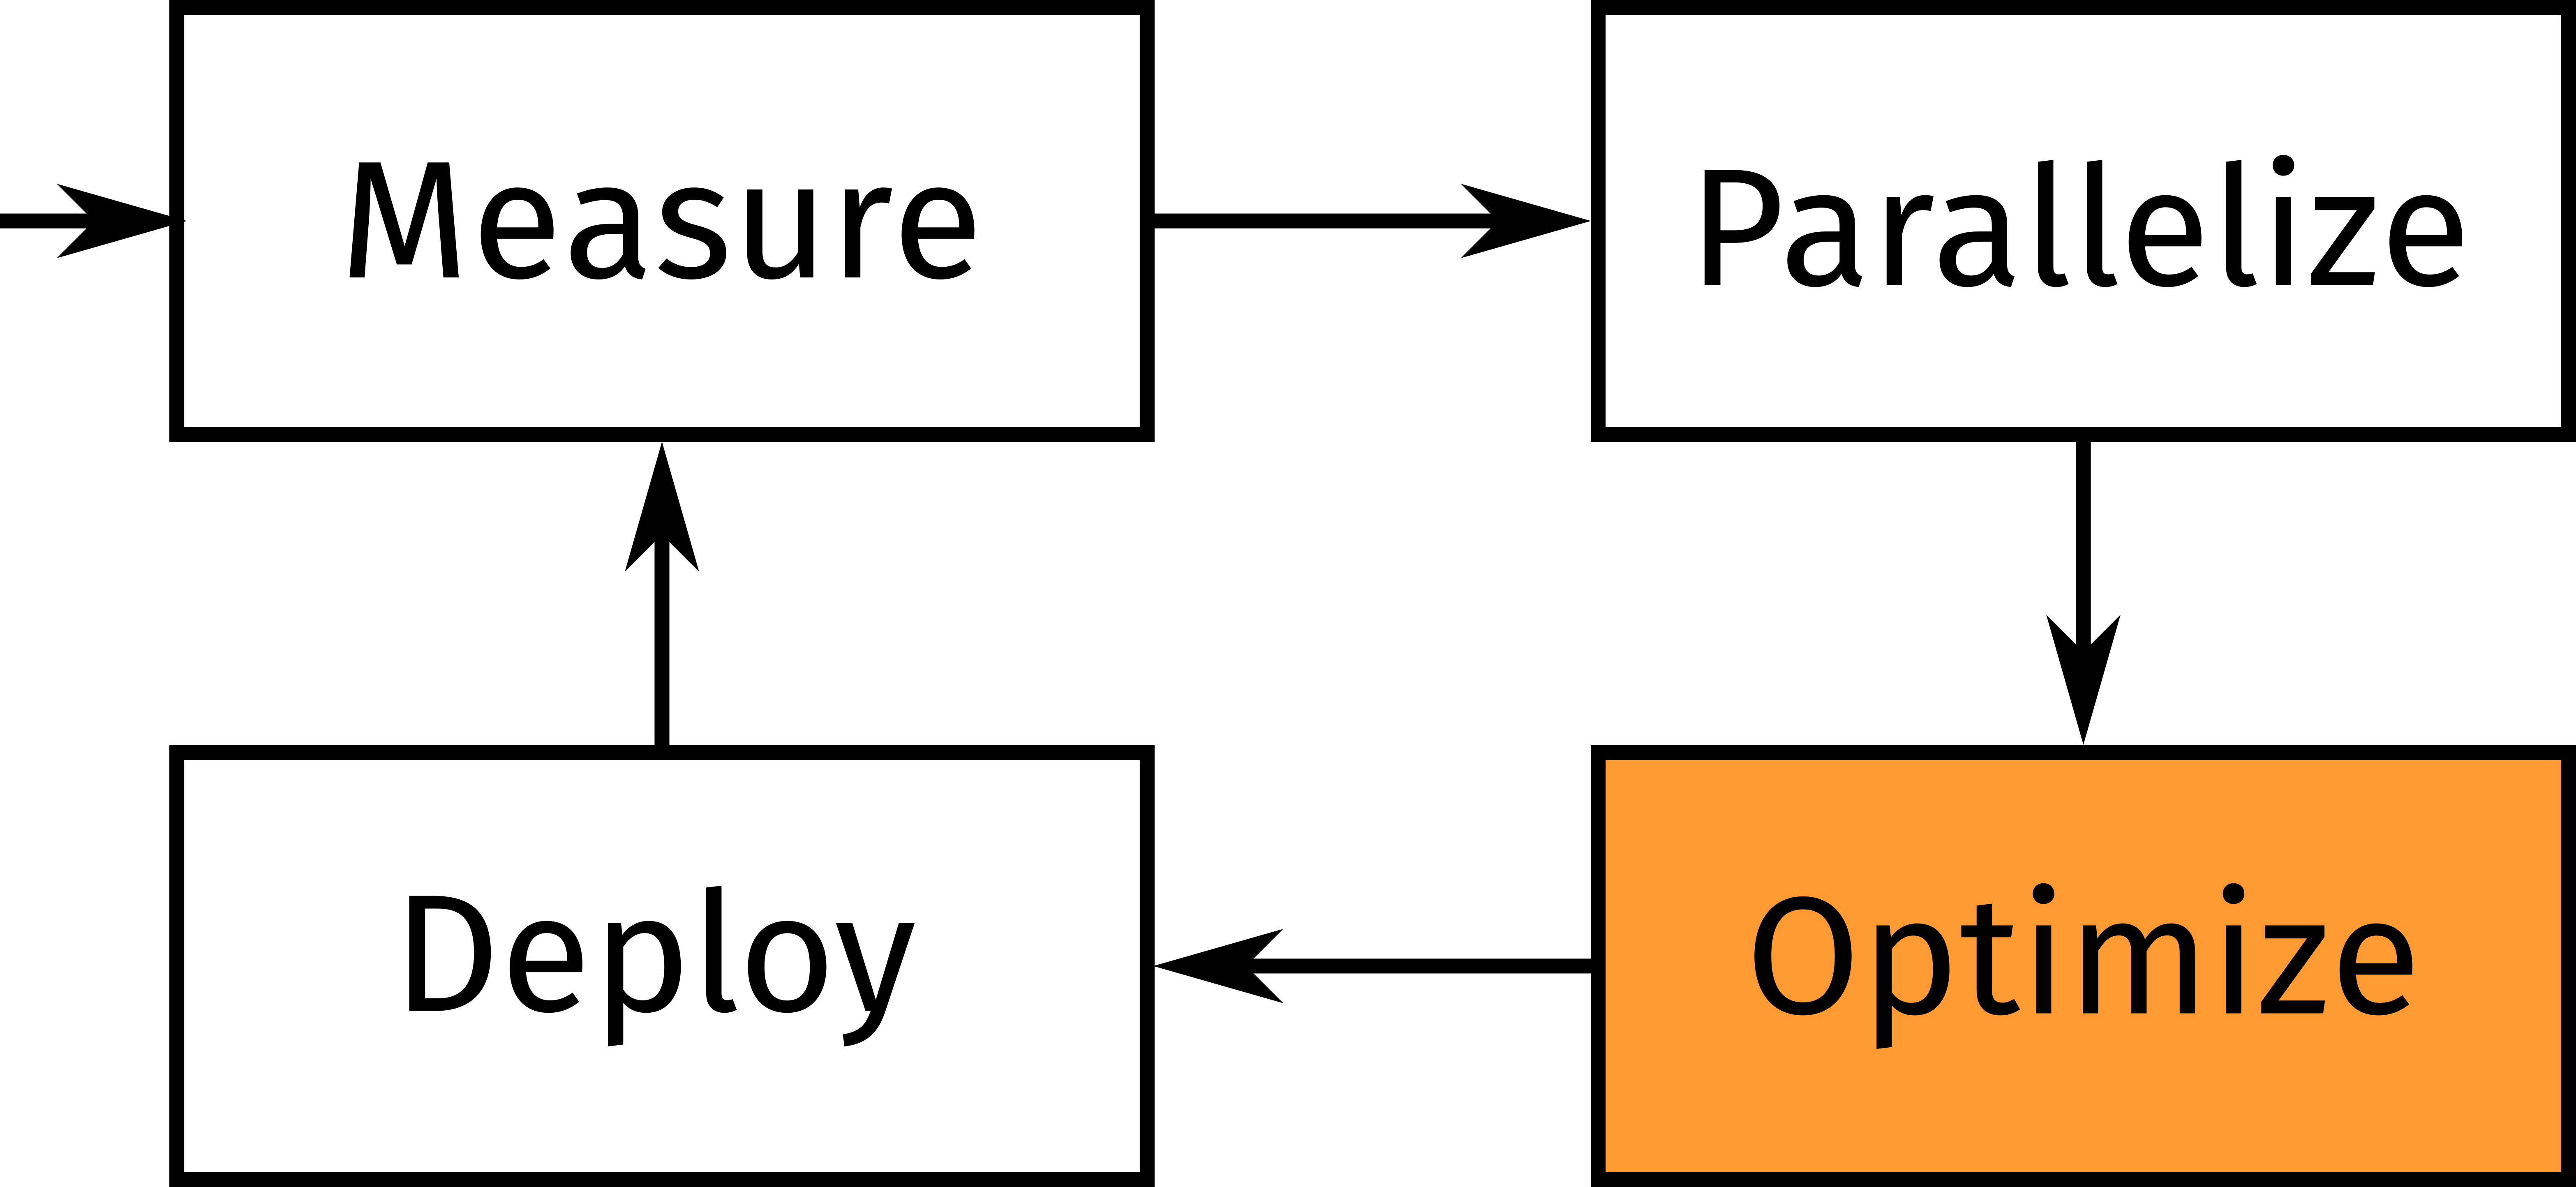
\includegraphics[width=.4\textwidth]{MPOD_O}
    \end{center}

    \vfill

    \pause
    Otimização:
    \begin{itemize}
        \item Processo \alert{cíclico} \pause e \alert{incremental}
            \pause
        \item Aplicável a \alert{diferentes níveis}
            \pause
        \item \alert{Ferramentas} são muito importantes
    \end{itemize}

    \pause
    \begin{center}
    \alert{Eficiência com algoritmos}, \pause \alert{desempenho com estruturas de dados}
    \end{center}
\end{frame}

\subsection{Deploy}

\begin{frame}
    \frametitle{Deploy}
    \begin{center}
    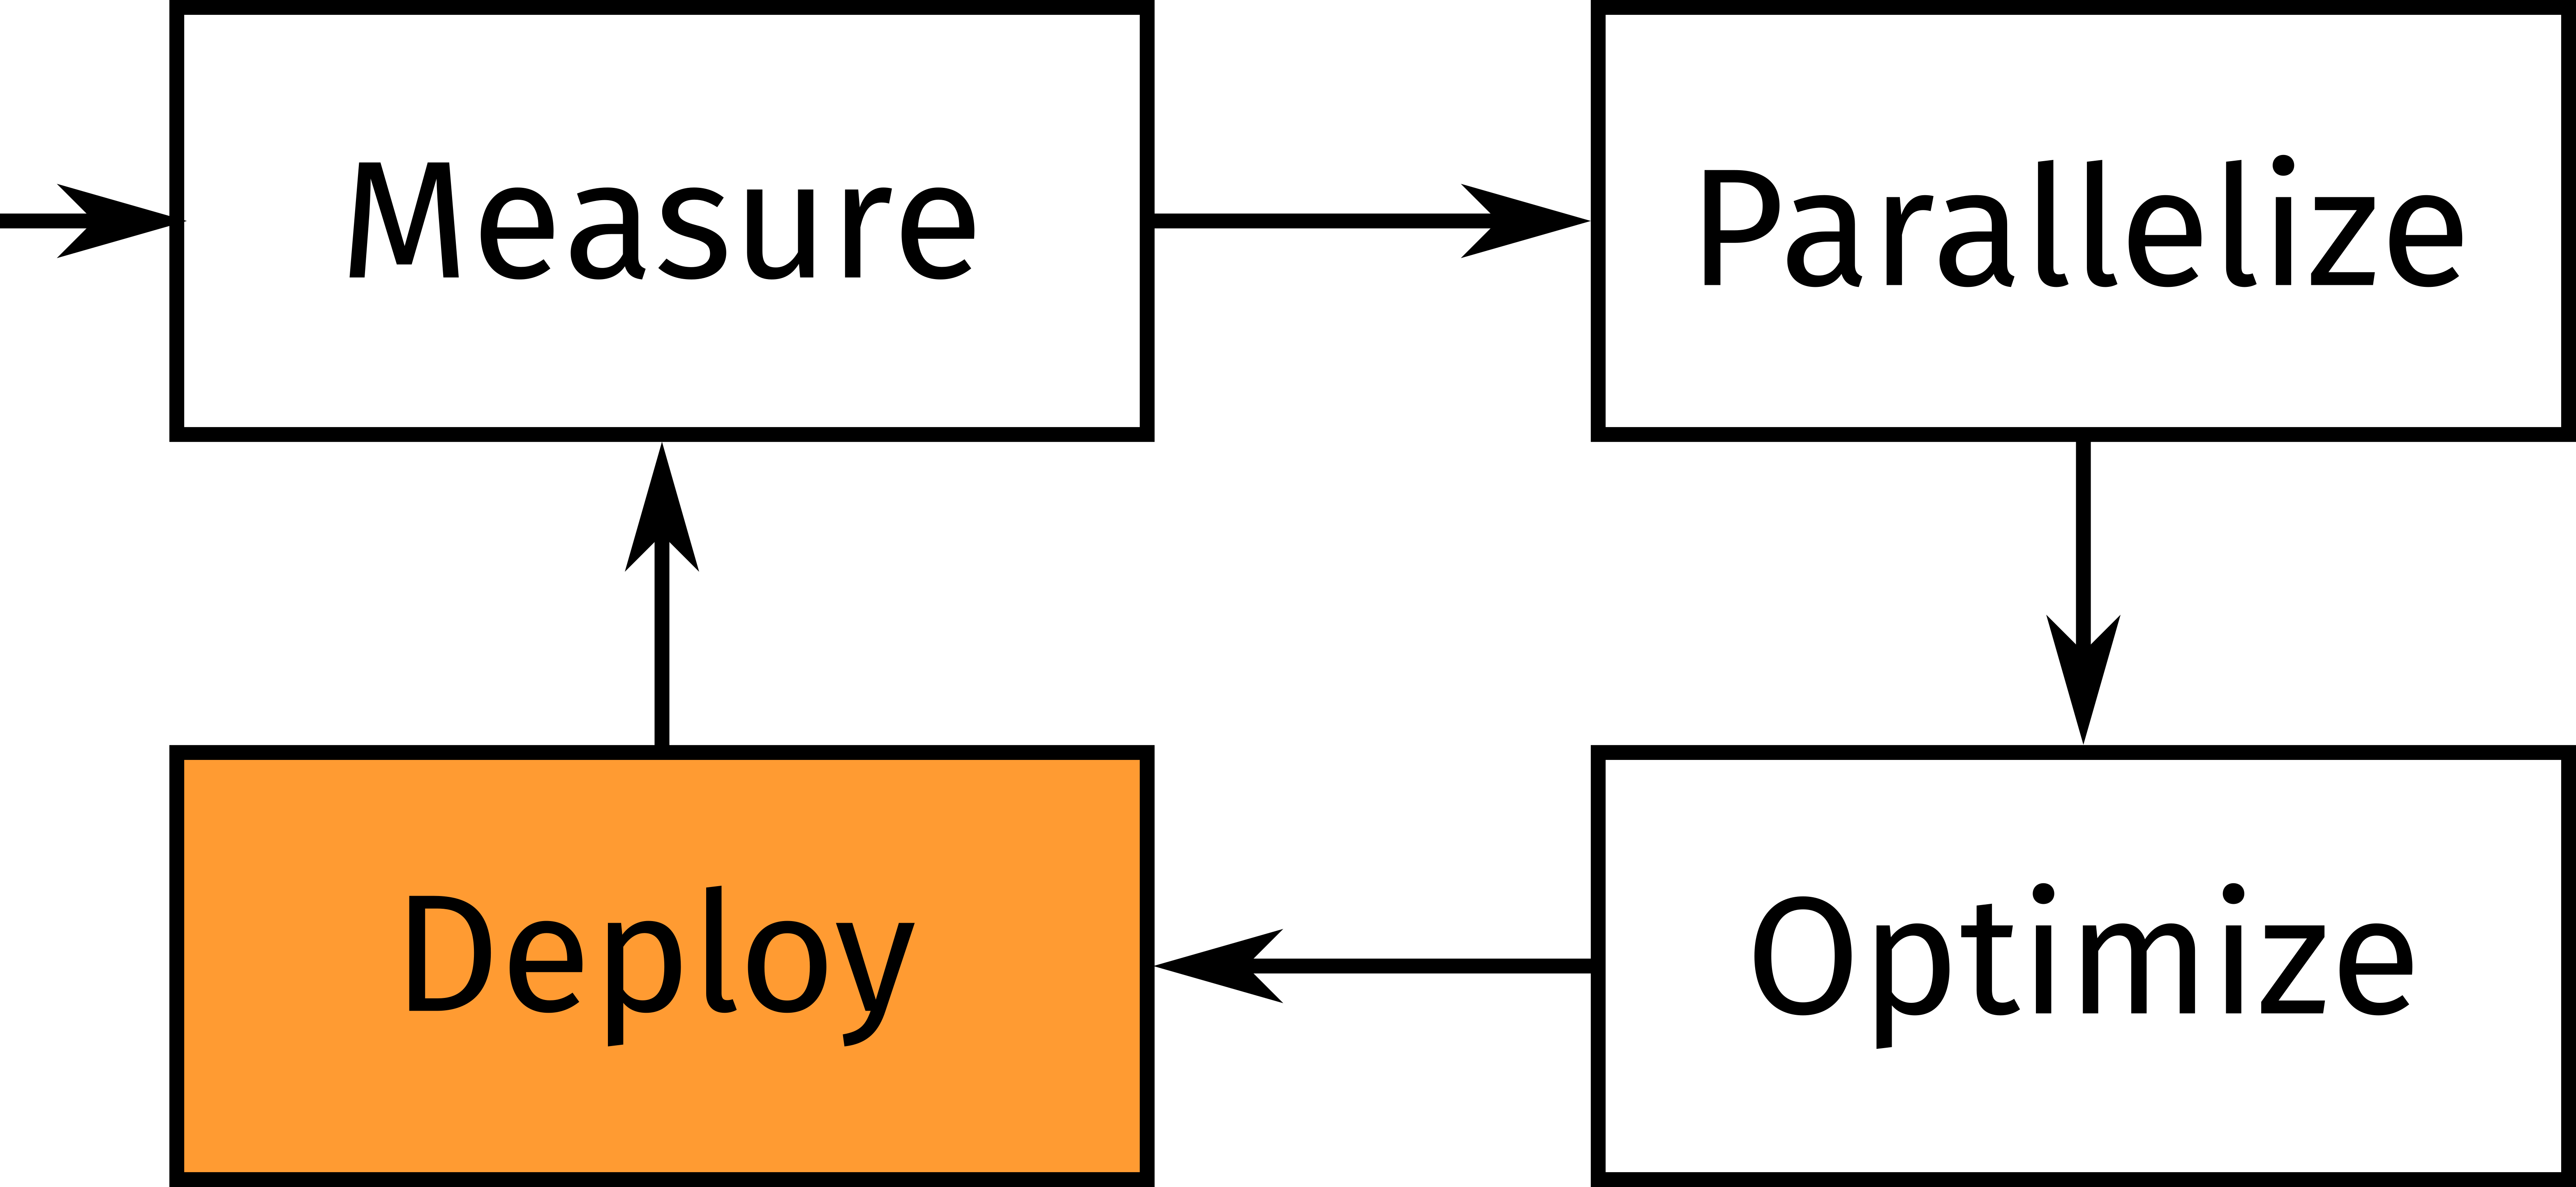
\includegraphics[width=.4\textwidth]{MPOD_D}
    \end{center}

    \vfill

    \pause
    \begin{itemize}
        \item Preparar a aplicação para a \alert{medição}
            \pause
        \item Otimizações e mudanças \alert{incrementais}
            \pause
        \item O quanto ainda é \alert{possível} otimizar?
    \end{itemize}
\end{frame}

\section{Análise de Aplicações CUDA}

\begin{frame}
    \frametitle{Análise de Aplicações CUDA}
    \begin{center}
        \includegraphics[width=.2\textwidth]{data_profile}
    \end{center}

    Computação \alert{paralela} e \alert{distribuída} é cada vez mais
    importante, mas \alert{código legado}:
    \pause
    \begin{itemize}
        \item \alert{Sequencial}
            \pause
        \item Paralelismo de \alert{baixa granularidade}
    \end{itemize}
    \pause

    Análise ou \alert{profiling}:
    \pause
    \begin{itemize}
        \item Quais são os \alert{hotspots} (\textit{gargalos}, \textit{bottlenecks})?
            \pause
        \item Podem ser paralelizados?
            \pause
        \item Quais \alert{workloads} são relevantes?
    \end{itemize}
\end{frame}

\subsection{Host e Device}

\begin{frame}
    \frametitle{\textit{Host} e \textit{Device}}
    Diferenças entre \textit{host} e \textit{device}:
    \begin{itemize}
        \item Modelo de \textit{threading}
            \pause
        \item Memória
    \end{itemize}

    \pause
    O que executar em \alert{GPUs}?
    \pause
    \begin{itemize}
        \item Grande quantidade de \alert{dados}
            \pause
        \item Operações \alert{independentes}
    \end{itemize}
    \pause

    Qual o impacto das \alert{transferências de dados}?
\end{frame}

\subsection{Profiling}

\begin{frame}
    \frametitle{\textit{Profiling}}
    Monitoramento de código \alert{em tempo de execução},
    obtendo informação para \alert{otimizar o código}
    \pause

    \alert{Instrumentação} do Código:
    \begin{itemize}
        \item Captura de \alert{eventos}
            \pause
        \item Geração de \alert{dados}
            \pause
        \item Ferramentas
    \end{itemize}
\end{frame}

\begin{frame}
    \frametitle{\textit{Profiling: Flamegraphs}}
    \begin{center}
        \includegraphics[width=\textwidth]{flamegraph}
    \end{center}

    Facilitam a análise de:
    \begin{itemize}
        \item \textit{Bottlenecks}, \textit{hotspots}, ou \textit{gargalos} de desempenho
            \pause
        \item Frequência e duração de \alert{chamadas de função}: \textit{On-CPU}
            \pause
        \item Tempo \alert{ocioso} (\textit{espera}): \textit{Off-CPU}
    \end{itemize}
\end{frame}

\begin{frame}
    \frametitle{Profiling: \texttt{nvprof}}
    \textit{Profiler} de \alert{linha de comando},
    permite a coleta de eventos relacionados a CUDA:
    \pause
    \begin{itemize}
        \item CPU e GPU
            \pause
        \item Execução do \textit{kernel}
            \pause
        \item Uso e transferência de memória
            \pause
        \item CUDA API
    \end{itemize}
    \pause

    Gera dados para \alert{posterior visualização}

    \begin{center}
        \tiny{Fonte: \url{docs.nvidia.com/cuda/profiler-users-guide} [Acessado em 29/07/16]}
    \end{center}
\end{frame}

\begin{frame}
    \frametitle{Profiling: \texttt{nvvp}}
    \centering
    \includegraphics[width=\textwidth]{nvvp}

    \vfill
    \tiny{Fonte: \url{docs.nvidia.com/cuda/profiler-users-guide} [Acessado em 29/07/16]}
\end{frame}

\begin{frame}
    \frametitle{Profiling: Ferramentas}
    \centering
    \includegraphics[width=.5\textwidth]{profile_tools}

    \vfill
    \tiny{Fonte: \url{developer.nvidia.com/performance-analysis-tools} [Acessado em 29/07/16]}
\end{frame}

\subsection{Debugging}

\begin{frame}
    \frametitle{\textit{Debugging}}
    Monitoramento de código \alert{em tempo de execução},
    obtendo informação para \alert{consertar erros} (\alert{bugs})
    \pause

    \alert{Instrumentação} do Código:
    \begin{itemize}
        \item Execução \alert{passo-a-passo}
            \pause
        \item \alert{Breakpoints}
            \pause
        \item Diferentes \alert{threads}
            \pause
        \item CUDA \texttt{\alert{gdb}} e \texttt{\alert{memcheck}}
    \end{itemize}
    \pause

    Facilitam a solução de:
    \begin{itemize}
        \item \alert{Vazamentos} de memória
            \pause
        \item Problemas com \alert{fluxo de controle}
            \pause
        \item ...
    \end{itemize}
\end{frame}

\section{Otimização de Aplicações CUDA}

\begin{frame}
    \frametitle{Otimização de Aplicações CUDA}
    \begin{center}
        \includegraphics[width=.2\textwidth]{optimization_icon}
    \end{center}

    Diferentes níveis de \alert{abstração} e \alert{prioridade}:
    \pause
    \begin{itemize}
        \item Memória
            \pause
        \item Fluxo de controle
            \pause
        \item Configuração de execução
            \pause
        \item Instruções
    \end{itemize}
\end{frame}

\subsection{Otimizações de Memória}

\begin{frame}
    \frametitle{Otimizações de Memória}
    São as \alert{mais importantes} para atingir \alert{alto desempenho}
    \pause

    Objetivos:
    \begin{itemize}
        \item Maximizar \alert{largura de banda} (\textit{bandwidth})
            \pause
        \item Minimizar \alert{transferências} entre \textit{device} e \textit{host}
            \pause
    \end{itemize}

    Boas práticas:
    \pause

    \begin{itemize}
        \item No \textit{device}:
            \pause
            \begin{itemize}
                \item Priorizar execução de \alert{computações}
                    \pause
                \item Criar e destruir \alert{estruturas de dados intermediárias}
                    \pause
                \item Accesos \alert{agrupados} (\textit{coalescentes}) à memória
            \end{itemize}
            \pause
        \item No \textit{host}:
            \pause
            \begin{itemize}
                \item Delegar execução de \alert{computações}
                    \pause
                \item Minimizar o número de \alert{transferências de dados}
            \end{itemize}
    \end{itemize}
\end{frame}

\subsection{Otimizações de Fluxo de Controle}

\begin{frame}
    \frametitle{Otimizações de Fluxo de Controle}
    \alert{Alta prioridade} para atingir \alert{alto desempenho}
    \pause

    Objetivos:
    \begin{itemize}
        \item Evitar \alert{divergência de fluxo de controle} dentro de
            \textit{warps}
            \pause
        \item \texttt{\alert{if}}, \texttt{\alert{switch}},
            \texttt{\alert{do}}, \texttt{\alert{for}}, \texttt{\alert{while}}
            \pause
        \item Fazer bom uso do \texttt{\alert{threadIdx}}
    \end{itemize}
\end{frame}

\subsection{Otimizações de Configuração de Execução}

\begin{frame}
    \frametitle{Otimizações de Configuração de Execução}
    Como aproveitar totalmente o potencial do \alert{device}?
    \pause
    \begin{itemize}
        \item Maximizar a \alert{ocupância}
            \pause
        \item Escolher bem os \alert{blocks} e \alert{threads}
            \pause
        \item Execução independente de \alert{kernels}
    \end{itemize}
\end{frame}

\subsection{Otimizações de Instruções}

\begin{frame}
    \frametitle{Otimizações de Instruções}
    \alert{Baixa prioridade} para atingir \alert{alto desempenho}:
    \pause
    \begin{itemize}
        \item \alert{Baixo nível}
            \pause
        \item Aplicadas a \alert{hotspots}
            \pause
        \item Feitas por \alert{experts}
        \item Após \alert{exaurir} outras possibilidades de otimização
            \pause
        \item \lq\lq{}\alert{Escovar \textit{bits}}\rq\rq{} \smiley{}
    \end{itemize}
\end{frame}

\section{Conclusão}

\begin{frame}
    \frametitle{Conclusão}
    \centering
        \includegraphics[width=.75\textwidth]{top500_accel}
    \vfill

    Atingir \alert{alto desempenho} através do uso de \alert{aceleradores} \pause (\alert{GPUs})
\end{frame}

\begin{frame}
    \frametitle{Conclusão}
    \begin{center}
        \includegraphics[width=.5\textwidth]{titan_x}
    \end{center}
    \vfill

    \pause
    Custo de \alert{implementação}, \alert{análise} e \alert{otimização}

    \pause
    \alert{Ferramentas} da plataforma \alert{CUDA}
\end{frame}

\subsection{Recursos}

\begin{frame}
    \frametitle{Recursos}
    O \emph{pdf} com as aulas e todo o código fonte estão no \alert{GitHub}:

    \begin{itemize}
        \item \url{github.com/phrb/intro-cuda}
    \end{itemize}

    Outros recursos:

    \begin{itemize}
        \item CUDA C: \url{docs.nvidia.com/cuda/cuda-c-programming-guide}
        \item CUDA Toolkit: \url{developer.nvidia.com/cuda-toolkit}
        \item Guia de Boas Práticas:
            \begin{itemize}
                \item \url{docs.nvidia.com/cuda/cuda-c-best-practices-guide}
            \end{itemize}
        \item GPU Teaching Kit: \url{syllabus.gputeachingkit.com}
        \item iPython: \url{ipython.org/notebook.html}
        \item Anaconda: \url{continuum.io/downloads}
    \end{itemize}
\end{frame}

\maketitle

\end{document}
